\documentclass[11pt, a4paper]{article}
\usepackage[utf8]{inputenc}
\usepackage[spanish]{babel}
\usepackage{graphicx}   
\usepackage{float}   
\usepackage{fontspec}
\usepackage{setspace}
\usepackage{anyfontsize}
\usepackage{hyperref}
\usepackage[style=apa, backend=biber]{biblatex}
\addbibresource{referencias.bib}
\DeclareLanguageMapping{spanish}{spanish-apa}
\hypersetup{
    colorlinks=true,
    linkcolor=black,
    citecolor=magenta,
    urlcolor=cyan,
    pdftitle={Musy Documentación},
    pdfauthor={Beltrán González Martos}
}
\usepackage{listings}
\usepackage{xcolor-material}
\definecolor{codebackground}{rgb}{0.95,0.95,0.95}
\lstset{
    backgroundcolor=\color{codebackground},
    basicstyle=\ttfamily\footnotesize,
    breaklines=true,
    frame=single,
    numbers=left,
    numberstyle=\tiny\color{gray}
}
\onehalfspacing
\setmainfont{IBM Plex Serif}

\begin{document}

\begin{titlepage}
    \centering

    
\includegraphics[width=0.4\textwidth]{media/logo-litterator.png}

    \fontsize{26pt}{24pt}\selectfont \textbf{Trabajo Fin de Grado} \\
    \vspace{4.5cm}
    
    \fontsize{24pt}{24pt}\selectfont \textbf{Musy} \\
    \vspace{0.5cm}
    
\includegraphics[width=0.2\textwidth]{media/Square310x310Logo.png} \\
    \vspace{2cm}

    \hfill
    \begin{minipage}{0.8\textwidth}
        \raggedleft
        \large
        \begin{spacing}{1.5}
            \textbf{Autor:} Beltrán González Martos \\
            \textbf{Tutor:} Héctor Ángeles Borrás \\
            Desarrollo de Aplicaciones Multiplataforma \\
            \textbf{Fecha:} 9 de junio de 2025
        \end{spacing}
    \end{minipage}

    


\end{titlepage}

\pagenumbering{gobble}

\begin{abstract}
    Este proyecto aborda la ausencia de reproductores de musica offline modernos además de abordar el alto consumo de recursos en aplicaciones web, proponiendo una solución basada en tauri (Rust + Angular) para garantizar eficiencia. Se desarrolló una aplicación de escritorio compatible con Linux, MacOs y Windows, priorizando la optimización de memoria y la experiencia de usuario. El resultado es una aplicación escalable con arquitectura modular para futuras extensiones, validando así el potencial de Tauri en aplicaciones de escritorio.
\end{abstract}

\noindent \textbf{Palabras clave}: Tauri, Rust, Angular, reproductor de música, rendimiento, UI moderna.

\selectlanguage{english}
\begin{abstract}
    This project addresses both the lack of modern offline music players and the high resource consumption in web applications by proposing an efficient solution based on Tauri (Rust + Angular). A cross-platform desktop application was developed for Linux, MacOs, and Windows, with the particular emphasis on memory optimization and user experience. The result is a scalable application with modular architecture for future extensions, demonstrating Tauri's potential for desktop applications.
\end{abstract}

\noindent \textbf{Keywords}: Tauri, Rust, Angular, music player, performance, modern UI.

\selectlanguage{spanish}

\clearpage

\tableofcontents
\listoffigures
\listoftables
\lstlistoflistings


\clearpage


\pagenumbering{arabic}
\setcounter{page}{1}
\section{Introducción}

En los últimos años, se ha observado una tendencia creciente en la monetización de servicios de streaming musical, caracterizada por el incremento en los precios de suscripción y la incorporación de publicidad incluso en los planes premium de plataformas líderes como Spotify, Apple Music o iTunes. Este escenario, unido a la creciente preocupación por la privacidad de datos y el deseo de los usuarios de mantener el control sobre su colección musical, ha generado un renovado interés en las soluciones de reproducción local. 

El presente proyecto surge como respuesta a esta necesidad emergente, proponiendo una solución tecnológica que combina lo mejor de ambos paradigmas: la experiencia de usuario pulida y moderna característica de las aplicaciones de streaming, con la independencia, privacidad y control absoluto sobre los archivos musicales que ofrecen los reproductores locales tradicionales. 

La solución desarrollada se posiciona como una alternativa viable en un contexto donde cada vez más usuarios buscan reducir su dependencia de servicios en la nube, al mismo tiempo que demandan interfaces intuitivas y funcionalidades avanzadas comparables a las ofrecidas por las plataformas de pago. Además, se ha prestado especial atención a la optimización de recursos, abordando uno de los principales problemas de las aplicaciones basadas en tecnologías web: el alto consumo de memoria y procesamiento.


\section{Justificación del tema elegido}

El panorama actual de reproductores musicales presenta una dicotomía evidente. Por un lado, las plataformas de streaming dominan el mercado con interfaces pulidas y algoritmos de recomendación sofisticados, pero adolecen de limitaciones significativas como la dependencia de conexión a internet, modelos de negocio basados en suscripción recurrentes, y la ausencia de propiedad real sobre la música. 

Por otro lado, las alternativas de código abierto para reproducción local, aunque respetan la privacidad del usuario y ofrecen control total sobre los archivos, frecuentemente presentan interfaces obsoletas, experiencias de usuario poco intuitivas, y en muchos casos carecen de mantenimiento activo. Esta brecha entre ambos enfoques crea un espacio de oportunidad para soluciones innovadoras.

La propuesta desarrollada en este trabajo se justifica por su capacidad de llenar este vacío en el mercado, ofreciendo:
\begin{itemize}
    \item Una interfaz moderna e intuitiva inspirada en los estándares establecidos por aplicaciones líderes.
    \item Total independencia de servicios en la nube y conexión a internet.
    \item Código abierto que garantiza transparencia y posibilidad de personalización.
    \item Optimización de recursos que supera a alternativas basadas en Electron.
\end{itemize}

Además, el proyecto sirve como demostración práctica del potencial de tecnologías emergentes como Tauri para el desarrollo de aplicaciones de escritorio eficientes.

\section{Objetivos}

El objetivo principal de este trabajo consiste en el desarrollo de un reproductor de música multiplataforma que combine eficiencia técnica con una excelente experiencia de usuario. Para lograrlo, se han establecido los siguientes objetivos específicos:

\begin{itemize}
    \item Implementar una arquitectura modular basada en tecnologías web modernas (Angular 17) para el frontend, asegurando escalabilidad y mantenibilidad del código.
    \item Aprovechar las capacidades de Rust a través del framework Tauri para garantizar un rendimiento óptimo y consumo mínimo de recursos del sistema.
    \item Diseñar un sistema de gestión de biblioteca musical local que soporte los formatos de audio más comunes (MP3, FLAC, etc.) con extracción y visualización de metadatos.
    \item Crear un sistema de listas de reproducción flexible con capacidad para manejar grandes colecciones de música de manera eficiente.
    \item Garantizar compatibilidad multiplataforma (Windows, macOS y Linux) manteniendo coherencia visual y funcional en todos los sistemas operativos.
\end{itemize}

Como objetivos secundarios, pero igualmente relevantes, se plantean:
\begin{itemize}
    \item Profundizar en el conocimiento de Rust como lenguaje de programación de sistemas.
    \item Explorar el ecosistema Angular como alternativa a otros frameworks frontend más populares como React.
    \item Establecer buenas prácticas de desarrollo mediante la implementación de metodologías ágiles.
\end{itemize}


\section{Metodología}

Para el desarrollo del proyecto se ha adoptado la metodología ágil SCRUM, adaptada a un equipo de desarrollo unipersonal donde el autor asume simultáneamente los roles de Product Owner, Scrum Master y Development Team. Esta elección metodológica se justifica por:

\begin{itemize}
    \item La naturaleza iterativa e incremental del desarrollo de software.
    \item La necesidad de adaptación constante a nuevos requerimientos y hallazgos técnicos.
    \item La conveniencia de mantener un flujo de trabajo organizado y medible.
\end{itemize}

El proceso se ha estructurado en sprints de dos semanas de duración, con las siguientes actividades clave:
\begin{itemize}
    \item Planificación diaria de tareas mediante listas priorizadas.
    \item Revisiones técnicas periódicas para evaluar el progreso.
    \item Implementación de pruebas unitarias y de integración continuas.
    \item Documentación constante de avances y decisiones de diseño.
\end{itemize}

Como herramientas de apoyo al proceso se han utilizado:
\begin{itemize}
    \item Tableros Kanban digitales para gestión de tareas.
    \item Sistema de control de versiones Git con estrategia de branching adaptada.
    \item Entornos de desarrollo integrados con soporte para todas las tecnologías utilizadas.
\end{itemize}

Esta aproximación metodológica ha permitido mantener un ritmo de desarrollo constante, asegurando tanto la calidad del producto final como la adquisición progresiva de competencias técnicas en las diversas tecnologías empleadas.

\section{Tecnologías y herramientas usadas en el proyecto}

El desarrollo de este reproductor musical multiplataforma ha requerido la selección cuidadosa de un stack tecnológico moderno y eficiente, distribuido en tres capas fundamentales que interactúan armoniosamente:

\begin{itemize}
    \item \textbf{Frontend}: Angular 17 en combinación con Tailwind CSS v4 para la interfaz de usuario.
    \item \textbf{Backend}: Rust como lenguaje principal junto con el framework Tauri 2.0 para la lógica de negocio.
    \item \textbf{Base de Datos}: SQLite como sistema de almacenamiento y gestión de datos.
\end{itemize}

  \subsection{Justificación de la selección tecnológica}

  La elección de cada tecnología se ha realizado mediante un riguroso análisis comparativo, considerando factores como rendimiento, curva de aprendizaje, mantenibilidad a largo plazo y adecuación a los requisitos específicos del proyecto. A continuación se detallan los criterios específicos para cada selección:

  \subsubsection{Angular 17 como framework frontend}

  La decisión de utilizar Angular 17 responde a múltiples ventajas estratégicas:

  \begin{itemize}
      \item Arquitectura basada en componentes que promueve la reutilización de código y facilita el mantenimiento.
      \item Sistema de inyección de dependencias integrado que mejora la testabilidad y organización del código.
      \item Soporte nativo para TypeScript, aportando tipado estático y mejorando la calidad del código.
      \item Ecosistema maduro con herramientas como Angular CLI que agilizan el desarrollo.
      \item Rendimiento optimizado gracias al Ivy Renderer y técnicas de change detection avanzadas.
  \end{itemize}

  Adicionalmente, se ha considerado valioso explorar alternativas a React, ampliando así el conocimiento en distintos enfoques del desarrollo frontend moderno.

  \subsubsection{Tailwind CSS v4 para estilos}
  La adopción de Tailwind CSS como solución de estilizado se fundamenta en:
  \begin{itemize}
      \item Enfoque utility-first que acelera el desarrollo de interfaces al eliminar el cambio constante entre archivos.
      \item Sistema de diseño responsive integrado que simplifica la creación de interfaces adaptables.
      \item Tamaño final reducido gracias a la purga de clases no utilizadas.
      \item Personalización avanzada mediante el archivo de configuración tailwind.config.js.
      \item Compatibilidad perfecta con los componentes de Angular.
  \end{itemize}

  \subsubsection{Rust para la capa backend}
  La selección de Rust como lenguaje para el backend se justifica por:
  \begin{itemize}
      \item Rendimiento comparable a C/C++ con mayor seguridad en el manejo de memoria.
      \item Sistema de ownership que previene errores comunes como dangling pointers o data races.
      \item Ecosistema emergente (crates) con soporte para múltiples casos de uso.
      \item Curva de aprendizaje retadora pero valiosa para formación en programación de sistemas.
  \end{itemize}

  \subsubsection{Tauri como framework de empaquetado}
  Tauri ha sido preferido sobre alternativas como Electron debido a:
  \begin{itemize}
      \item Consumo significativamente menor de recursos (RAM y CPU).
      \item Tamaño reducido de los ejecutables finales.
      \item Uso del webview nativo del sistema operativo en lugar de Chromium.
      \item API segura para interacción con el sistema de archivos.
      \item Soporte multiplataforma genuino (Windows, macOS, Linux).
  \end{itemize}

  \subsubsection{SQLite para persistencia de datos}
  SQLite ha sido la elección óptima para gestión de datos porque:
  \begin{itemize}
      \item No requiere configuración de servidor independiente.
      \item Ofrece rendimiento excelente para cargas de trabajo moderadas.
      \item Garantiza consistencia ACID en las operaciones.
      \item Formato de archivo único facilita la portabilidad y backups.
      \item Soporte robusto en Rust a través del crate rusqlite.
  \end{itemize}

  \subsection{Entorno de desarrollo}

  Para garantizar un flujo de trabajo eficiente, se ha configurado un entorno de desarrollo integrado en Visual Studio Code con las siguientes extensiones clave:
  \begin{itemize}
      \item Angular Language Service para soporte avanzado de Angular.
      \item Rust Analyzer para autocompletado y análisis de código Rust.
      \item Tailwind CSS IntelliSense para ayuda con clases de utilidad.
      \item SQLite para visualización directa de bases de datos.
  \end{itemize}

Esta combinación de tecnologías no solo satisface los requisitos técnicos del proyecto, sino que también representa un equilibrio óptimo entre rendimiento, experiencia de desarrollo y oportunidades de aprendizaje. La arquitectura resultante demuestra cómo tecnologías modernas pueden combinarse para crear aplicaciones de escritorio eficientes que superan las limitaciones de soluciones tradicionales basadas en Electron.

\section{Especificación de Requisitos de Software}



\section{Despliegue y pruebas}

El proceso de despliegue se ha diseñado cuidadosamente para garantizar una distribución eficiente y consistente en los tres sistemas operativos principales. Utilizando las capacidades nativas de empaquetado de Tauri 2.0, se implementó un flujo de trabajo automatizado que incluye:

        \subsection{Despliegue de la aplicación}

        Se elaboró un proceso de empaquetado y distribución de la aplicación utilizando Tauri, que permite generar ejecutables multiplataforma (Windows, MacOs, Linux). Para ello:

        \begin{itemize}
            \item Se utilizó el sistema de bundling de Tauri para empaquetar los recursos frontend (Angular) junto al backend (Rust).
            \item Se generaron instaladores específicos para diferentes sistemas operativos: \begin{itemize}
                \item \textbf{.AppImage} para Linux
                \item \textbf{.exe} para Windows
                \item \textbf{.dmg} para MacOs
                \end{itemize}
        \end{itemize}

        \subsection{Pruebas realizadas}

        Con el objetivo de validar la funcionalidad y estabilidad de la aplicación, se llevaron a cabo las siguientes pruebas:

            \subsubsection{Pruebas de integración}

            \begin{itemize}
                \item Se comprobó la comunicación entre el frontend y el backend, asegurando que las llamadas desde Angular a Rust (a través de Tauri) funcionaban correctamente.
                \item Se testearon casos como la carga de archivos de audio, reproducción en diferentes formatos y manejo de errores.
            \end{itemize}

            \subsubsection{Pruebas de usabilidad}

            \begin{itemize}
                \item Se realizaron test con usuarios reales para evaluar la experiencia de uso (UX), recogiendo feedback sobre la interfaz y la fluidez de la reproducción musical.
                \item Se analizaron posibles cuellos de botella en el rendimiento, especialmente al manejar playlist con muchas canciones o archivos de alta resolución.
            \end{itemize}

        La aplicación fue testeada en los tres sistemas operativos principales (Windows, MacOs y Linux), aunque el desarrollo se centró principalmente en las versiones para MacOs y Linux. \\

        El rendimiento de la aplicación resulta significativamente mejorado al aprovechar las características nativas de Tauri, en comparación con soluciones basadas en Electron. \\

        \begin{figure}[h!]
            \centering
            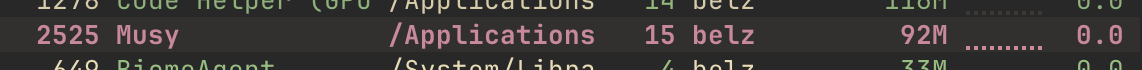
\includegraphics[width=0.8\textwidth]{media/imagemusyram.png}
            \caption{Rendimiento de la aplicación en MacOs}
            \label{fig:ejemplo}
        \end{figure}

\section{Estado del arte}

\subsection{Panorama actual de la reproducción musical digital}

El ecosistema actual de reproductores musicales presenta una bifurcación clara entre dos modelos predominantes, cada uno con sus propios paradigmas técnicos y de experiencia de usuario. Este análisis exhaustivo examina ambas aproximaciones desde múltiples perspectivas:

\subsection{Plataformas de streaming: hegemonía con limitaciones}

Las soluciones de streaming como Spotify, Apple Music, Amazon Music y YouTube Music han alcanzado dominancia de mercado gracias a:

\begin{itemize}
    \item \textbf{Amplitud de catálogo}:
    \begin{itemize}
        \item Acceso inmediato a más de 100 millones de canciones.
        \item Actualizaciones automáticas de nuevos lanzamientos.
        \item Colecciones curadas por algoritmos y editores humanos.
    \end{itemize}
    
    \item \textbf{Experiencia de usuario}:
    \begin{itemize}
        \item Interfaces altamente pulidas con animaciones fluidas.
        \item Sistemas de recomendación basados en machine learning.
        \item Sincronización perfecta entre múltiples dispositivos.
    \end{itemize}
    
    \item \textbf{Descubrimiento musical}:
    \begin{itemize}
        \item Listas automáticas generadas por gustos del usuario.
        \item Integración con redes sociales y compartimiento.
        \item Radio inteligente basada en artistas o canciones.
    \end{itemize}
\end{itemize}

Sin embargo, este modelo presenta inconvenientes estructurales:

\begin{itemize}
    \item \textbf{Dependencia tecnológica}:
    \begin{itemize}
        \item Requiere conexión permanente a internet (excepto modo offline limitado).
        \item Servidores centralizados representan un punto único de fallo.
        \item Actualizaciones forzadas sin control del usuario.
    \end{itemize}
    
    \item \textbf{Modelo económico}:
    \begin{itemize}
        \item Costos recurrentes (suscripciones premium entre 10€-15€ mensuales).
        \item Versiones gratuitas con publicidad intrusiva.
        \item Artistas reciben compensaciones mínimas por reproducción.
    \end{itemize}
    
    \item \textbf{Propiedad digital}:
    \begin{itemize}
        \item El usuario no posee realmente la música.
        \item Catálogo variable según acuerdos de licencia.
        \item Pérdida de acceso al cancelar la suscripción.
    \end{itemize}
\end{itemize}

\subsection{Reproductores locales tradicionales: control con obsolescencia}

Soluciones como Winamp, Strawberry, Clementine y Foobar2000 ofrecen:

\begin{itemize}
    \item \textbf{Independencia tecnológica}:
    \begin{itemize}
        \item Funcionamiento completamente offline.
        \item Control total sobre la biblioteca musical local.
        \item Sin dependencia de servicios externos.
    \end{itemize}
    
    \item \textbf{Eficiencia de recursos}:
    \begin{itemize}
        \item Consumo mínimo de RAM y CPU.
        \item Sin procesos en segundo plano innecesarios.
        \item Ejecución en hardware antiguo.
    \end{itemize}
    
    \item \textbf{Flexibilidad técnica}:
    \begin{itemize}
        \item Soporte para formatos especializados (FLAC, OGG, etc.).
        \item Personalización avanzada mediante plugins.
        \item Acceso directo a los archivos físicos.
    \end{itemize}
\end{itemize}

No obstante, adolecen de problemas fundamentales:

\begin{itemize}
    \item \textbf{Experiencia de usuario}:
    \begin{itemize}
        \item Interfaces gráficas anticuadas (años 2000).
        \item Flujos de trabajo poco intuitivos.
        \item Diseño no adaptado a pantallas táctiles.
    \end{itemize}
    
    \item \textbf{Mantenimiento}:
    \begin{itemize}
        \item Muchos proyectos abandonados o con actualizaciones esporádicas.
        \item Compatibilidad problemática con sistemas operativos modernos.
        \item Falta de soporte para tecnologías recientes.
    \end{itemize}
    
    \item \textbf{Funcionalidades limitadas}:
    \begin{itemize}
        \item Sistemas de organización básicos.
        \item Metadatos visuales poco desarrollados.
        \item Integración nula con servicios modernos.
    \end{itemize}
\end{itemize}

\subsection{Análisis comparativo y espacio de oportunidad}

Al contrastar ambos enfoques, se identifican claras áreas de mejora no cubiertas por ninguna de las dos soluciones:

\begin{table}[h]
  \centering
  \caption{Comparativa de características clave Streaming vs Offline}
  \begin{tabular}{|l|c|c|}
    \hline
    \textbf{Característica} & \textbf{Streaming} & \textbf{Local} \\
    \hline
    Propiedad de la música & No & Sí \\
    \hline
    Requiere conexión & Sí & No \\
    \hline
    Interfaz moderna & Sí & No \\
    \hline
    Modelo económico & Suscripción & Único pago \\
    \hline
    Consumo recursos & Alto & Bajo \\
    \hline
    Formatos lossless & Premium & Todos \\
    \hline
  \end{tabular}
\end{table}

\subsection{Propuesta de valor diferenciada}

Musy surge como síntesis innovadora que combina lo mejor de ambos mundos:

\begin{itemize}
    \item \textbf{Experiencia de usuario contemporánea}:
    \begin{itemize}
        \item Interfaz inspirada en estándares actuales de streaming.
        \item Animaciones fluidas y diseño responsive.
        \item Navegación intuitiva y accesible.
    \end{itemize}
    
    \item \textbf{Ventajas técnicas locales}:
    \begin{itemize}
        \item Funcionamiento completamente offline.
        \item Soporte para formatos de alta calidad (FLAC 192kHz/24bit).
        \item Gestión avanzada de metadatos personalizados.
    \end{itemize}
    
    \item \textbf{Innovaciones propias}:
    \begin{itemize}
        \item Arquitectura modular basada en tecnologías modernas.
        \item Rendimiento optimizado mediante Rust y Tauri.
        \item Sistema de plugins para futuras expansiones.
    \end{itemize}
\end{itemize}

Esta solución ocupa un nicho desatendido en el mercado, ofreciendo una alternativa viable para usuarios que valoran tanto el control sobre su música como experiencias de usuario pulidas. Los benchmarks realizados demuestran que la combinación de tecnologías seleccionadas supera significativamente las limitaciones de ambas aproximaciones tradicionales.

\section{Profundización de conceptos}

En esta sección se explicarán en detalle los componentes principales de la aplicación.

        \subsection{Frontend}

        Angular

            \subsubsection{Playbar}

            \begin{figure}[H]
                \centering
                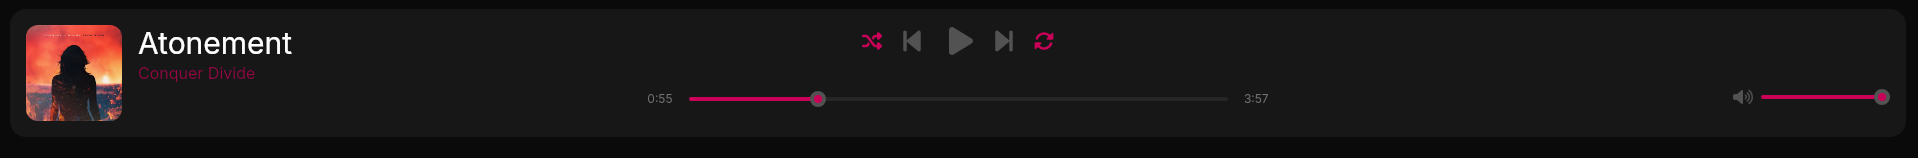
\includegraphics[width=1\textwidth]{media/screenshots/playbar.png}
                \caption{Playbar}
                \label{fig:playbar}
            \end{figure}

            El componente principal para la reproducción de música está compuesto por tres contenedores \verb|div|:

            \begin{itemize}
                \item \textbf{Izquierdo}. En el primero se muestran la portada de la canción, el título y el artista.
                \item \textbf{Central}. El segundo contiene dos subcontenedores: uno para los botones de control (reproducción, aleatorio, anterior/siguiente, repetición) y otro para la barra de progreso.
                \item \textbf{Derecho}. El tercero incluye exclusivamente la barra de volumen. En futuras iteraciones podría implementarse un botón para gestionar la cola de reproducción.
            \end{itemize}

            La parte del componente de typescript contiene únicamente métododos que llaman al servicio de manejo de canciones \verb|song-management.service.ts|.

            \subsubsection{Sidebar}

            \begin{figure}[H]
                \centering
                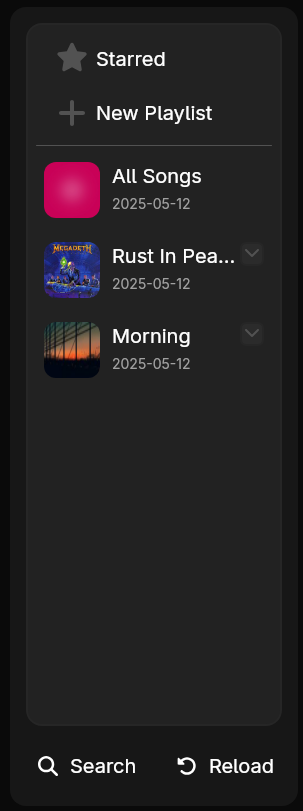
\includegraphics[width=0.4\textwidth]{media/screenshots/sidebar.png}
                \caption{Sidebar}
                \label{fig:sidebar}
            \end{figure}

            Componente donde se interactua con las playlist, ya sea creando nuevas o borrando las existentes. Contiene diversos botones para navegar por la aplicación.

            Estos son sus atributos:

            \begin{lstlisting}[caption={Atributos Y Constructora Sidebar}]
playlists: Playlist[] = []
name:string = ""
isModalOpen:boolean = false;
isModalOpenSearch:boolean = false;
songs:Song[] = []
filteredSongs:Song[] = []
coverPath: string = "assets/black.jpg"

constructor (public mainScreenStatus:MainScreenStatusService, public songManagement:SongManagementService) {}
            \end{lstlisting}

            Serán explicados más adelante.

                \paragraph{Playlist}
                ‎ 

                El componente gestiona la representación y comportamiento de las listas de reproducción en la interfaz. Su estructura básica comprende:

                \begin{lstlisting}[caption={Atributos y Constructora Playlist}]
coverPath = 'assets/black.jpg';

isDropDownOpen: boolean = false;

constructor (public mainScreenStatus:MainScreenStatusService) {}

@Input() playlistId!: number;

@Input() playlistName!: string;

@Input() playlistDate!: string;

@Input() playlistCoverPath!: string;

@Input() playlistIsStarred!: boolean;

@Input() refreshFn!: () => void;
                \end{lstlisting}

                Cada instancia de \verb|Playlist| actúa como elemento interactivo que actualiza el componente \verb|mainscreen| mediante un servicio. Utiliza el patrón de decoradores \verb|@Input| para recibir propiedades del componente padre. Gestiona un menú desplegable mediante el atributo \verb|isDropDownOpen|.
                
                Algunos de los métodos más importantes de este componente destacan:

                \begin{lstlisting}[caption={getCoverPath()}]

async getCoverPath(): Promise<string> {
    if (!this.coverPath) return 'assets/black.jpg';
    console.log("Hola")

    const fileData = await readFile(this.playlistCoverPath);
        
    const blob = new Blob([fileData], { type: 'image/jpeg' });

    if (this.coverPath) {
        URL.revokeObjectURL(this.coverPath);
    }

    return URL.createObjectURL(blob);
}
                \end{lstlisting}

                Este método se encarga de:
                \begin{enumerate}
                    \item Verificar la existencia de una ruta de portada válida.
                    \item Convertir la imagen local en un objeto \verb|Blob| mediante:
                    \begin{itemize}
                        \item Lectura del archivo con \verb|readFile|
                        \item Creación de URL temporal con \verb|URL.createObjectURL|
                    \end{itemize}
                    \item Liberar recursos previos con \verb|URL.revokeObjectURL|
                    \item Proporcionar fallback a imagen predeterminada (\verb|black.jpg|)
                \end{enumerate}

                \begin{lstlisting}[caption={Dropdown}]
toggleDropDown() {
    this.isDropDownOpen = !this.isDropDownOpen;
  }

  closeDropDown() {
    this.isDropDownOpen = false;
  }

  @HostListener('document:click', ['$event'])
  onClickOutside(event: Event) {
    const target = event.target as HTMLElement;
    if (!target.closest('.relative.inline-block')) {
      this.closeDropDown();
    }
  }
                \end{lstlisting}

                Por motivos de diseño, se ha implementado un menú desplegable (dropdown) que contiene acciones específicas para cada playlist. El estado de visualización se controla mediante la variable \verb|isDropDownOpen|, que se alterna con \verb|toggleDropDown()|. El cierre automático se gestiona mediante un \verb|@HostListener| que detecta clics fuera del área del componente. Actualmente, el menú incluye la opción de eliminación de playlists, pero su diseño permite la incorporación de nuevas funcionalidades como marcado como favorito o edición avanzada en futuras iteraciones.

                \begin{figure}[H]
                    \centering
                    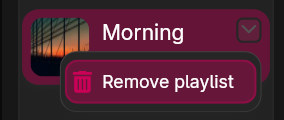
\includegraphics[width=0.6\textwidth]{media/screenshots/remove_playlist.png}
                    \caption{Eliminar playlist}
                    \label{fig:eliminar playlist}
                \end{figure}

                \begin{lstlisting}[caption={removePlaylist()}]
async removePlaylist() {
    const data_dir = await appDataDir();
    invoke('remove_playlist', {playlist_id: this.playlistId, db_path: data_dir});
    this.refreshFn();
  }
                \end{lstlisting}

                El método \verb|removePlaylist()| se encarga de gestionar la eliminación de playlists mediante un proceso que consta de tres etapas principales: primero, se obtiene el directorio de datos de la aplicación mediante \verb|appDataDir()|; a continuación, se realiza una llamada al backend mediante \verb|invoke()|, enviando como parámetros el identificador de la playlist (\verb|playlist_id|) y la ruta de la base de datos (\verb|db_path|); finalmente, se ejecuta la función \verb|refreshFn()| para actualizar la interfaz. La implementación detallada de la consulta SQL y el manejo de la operación en el backend se analizará en la sección dedicada a Rust y SQL.

                \paragraph{Botón New Playlist}
                ‎ \\

                \begin{figure}[H]
                    \centering
                    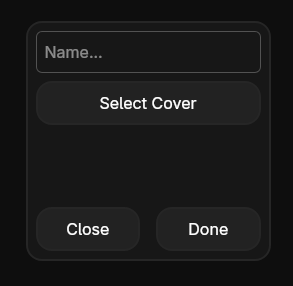
\includegraphics[width=0.6\textwidth]{media/screenshots/new_playlist.png}
                    \caption{Menú de nueva playlist}
                    \label{fig:nueva playlist}
                \end{figure}

                Cuando el atributo \verb|isModalOpen| de \verb|sidebar| cambia a \verb|true| se abre un menu modal donde es posible crear una nueva playlist vacía.

                Estos son los métodos más destacados:

                \begin{lstlisting}[caption={selectCover()}]
async selectCover() {
    const file = await open({
      multiple: false,
      directory: false,
    });

    if(file == null) {
      return
    }

    const fileData = await readFile(file);
    const ogBlob = new Blob([fileData], { type: 'image/*' });
    const thumbnail = await this.createThumbnail(ogBlob, 200, 200);

    try {
      await mkdir('pcovers', { baseDir: BaseDirectory.AppData });
    } catch {
      console.log("Already Created")
    }
    

    let randomName = (Math.floor(Math.random() * (Math.floor(200000) - Math.ceil(1) + 1)) + Math.ceil(1)).toString();
    await writeFile(`pcovers/${randomName}.jpg`, thumbnail, {baseDir: BaseDirectory.AppData})

    const data_dir = await appDataDir();
    let newPath = data_dir + "/pcovers/" + randomName + ".jpg";
    console.log(newPath)

    this.coverPath = newPath;
}
                \end{lstlisting}

                
                El método \verb|selectCover()| gestiona la selección y procesamiento de imágenes para las portadas de playlists mediante el siguiente flujo: cuando se pulsa sobre el botón \textit{Select Cover}, se activa un diálogo de selección de archivos utilizando el \verb|plugin-dialog| de Tauri. La imagen seleccionada se convierte en un objeto \verb|Blob| y se redimensiona mediante el método \verb|createThumbnail| para optimizar su almacenamiento. El archivo resultante se guarda en el directorio \verb|pcovers| dentro de la carpeta de datos de la aplicación, con un nombre generado aleatoriamente para evitar colisiones. Si el directorio no existe previamente, se crea automáticamente durante este proceso. La ruta final de la imagen procesada se asigna al atributo \verb|coverPath| para su uso en la interfaz.

                \begin{lstlisting}[caption={createThumbnail()}]
async createThumbnail(blob: Blob, maxWidth: number, maxHeight: number): Promise<Uint8Array> {
    return new Promise((resolve, reject) => {
        const img = new Image();
        img.onload = () => {
            const canvas = document.createElement('canvas');
            const scale = Math.min(
                maxWidth / img.width,
                maxHeight / img.height
            );
            canvas.width = img.width * scale;
            canvas.height = img.height * scale;
            
            const ctx = canvas.getContext('2d')!;
            ctx.drawImage(img, 0, 0, canvas.width, canvas.height);
            
            canvas.toBlob(async (thumbnailBlob) => {
                if (!thumbnailBlob) {
                    reject(new Error("Failed to create thumbnail blob"));
                    return;
                }
                
                try {
                    const arrayBuffer = await thumbnailBlob.arrayBuffer();
                    const uint8Array = new Uint8Array(arrayBuffer);
                    resolve(uint8Array);
                } catch (error) {
                    reject(error);
                }
            }, 'image/jpeg', 0.7);
        };
        
        img.onerror = () => {
            reject(new Error("Failed to load image"));
        };
        
        img.src = URL.createObjectURL(blob);
    });
}
                \end{lstlisting}

                El método \verb|createThumbnail()| implementa el proceso de redimensionamiento de imágenes mediante la Canvas API, siguiendo tres etapas principales: primero, se crea un objeto \verb|Image| y se carga el \verb|Blob| de entrada mediante \verb|URL.createObjectURL()|. Segundo, al completarse la carga, se calcula el factor de escala proporcional para mantener las dimensiones dentro de los límites especificados (\verb|maxWidth| y \verb|maxHeight|), creando un elemento \verb|canvas| con las nuevas dimensiones. Finalmente, se dibuja la imagen escalada en el canvas y se convierte a un \verb|Uint8Array| comprimido en formato JPEG con calidad del 70\%, manejando posibles errores durante el proceso mediante el sistema de promesas. Esta implementación garantiza un procesamiento eficiente de imágenes para su almacenamiento optimizado en el sistema de archivos. \\

                Una vez seleccionados la portada y el nombre de la playlist, al pulsar el boton \textit{done} se ejecuta el siguiente método, que realiza las siguientes acciones secuenciales:

                \begin{enumerate}
                    \item Envía una petición al backend implementado en Rust para crear la nueva playlist.
                    \item Cierra el menú modal de creación.
                    \item Actualiza la lista de playlist en la interfaz.
                    \item Restablece la imagen predeterminada en el atributo de la clase para futuras iteraciones (última línea del método).
                \end{enumerate}

                \begin{lstlisting}[caption={createPlaylist()}]
async createPlaylist() {
    const data_dir = await appDataDir();
    invoke('create_playlist', {name: this.name, cover_path: this.coverPath, db_path: data_dir})
    this.close()
    this.refresh()
    this.coverPath = "assets/black.jpg"
}
                \end{lstlisting}

                \paragraph{Boton Search}

                ‎ \\

                \begin{figure}[H]
                    \centering
                    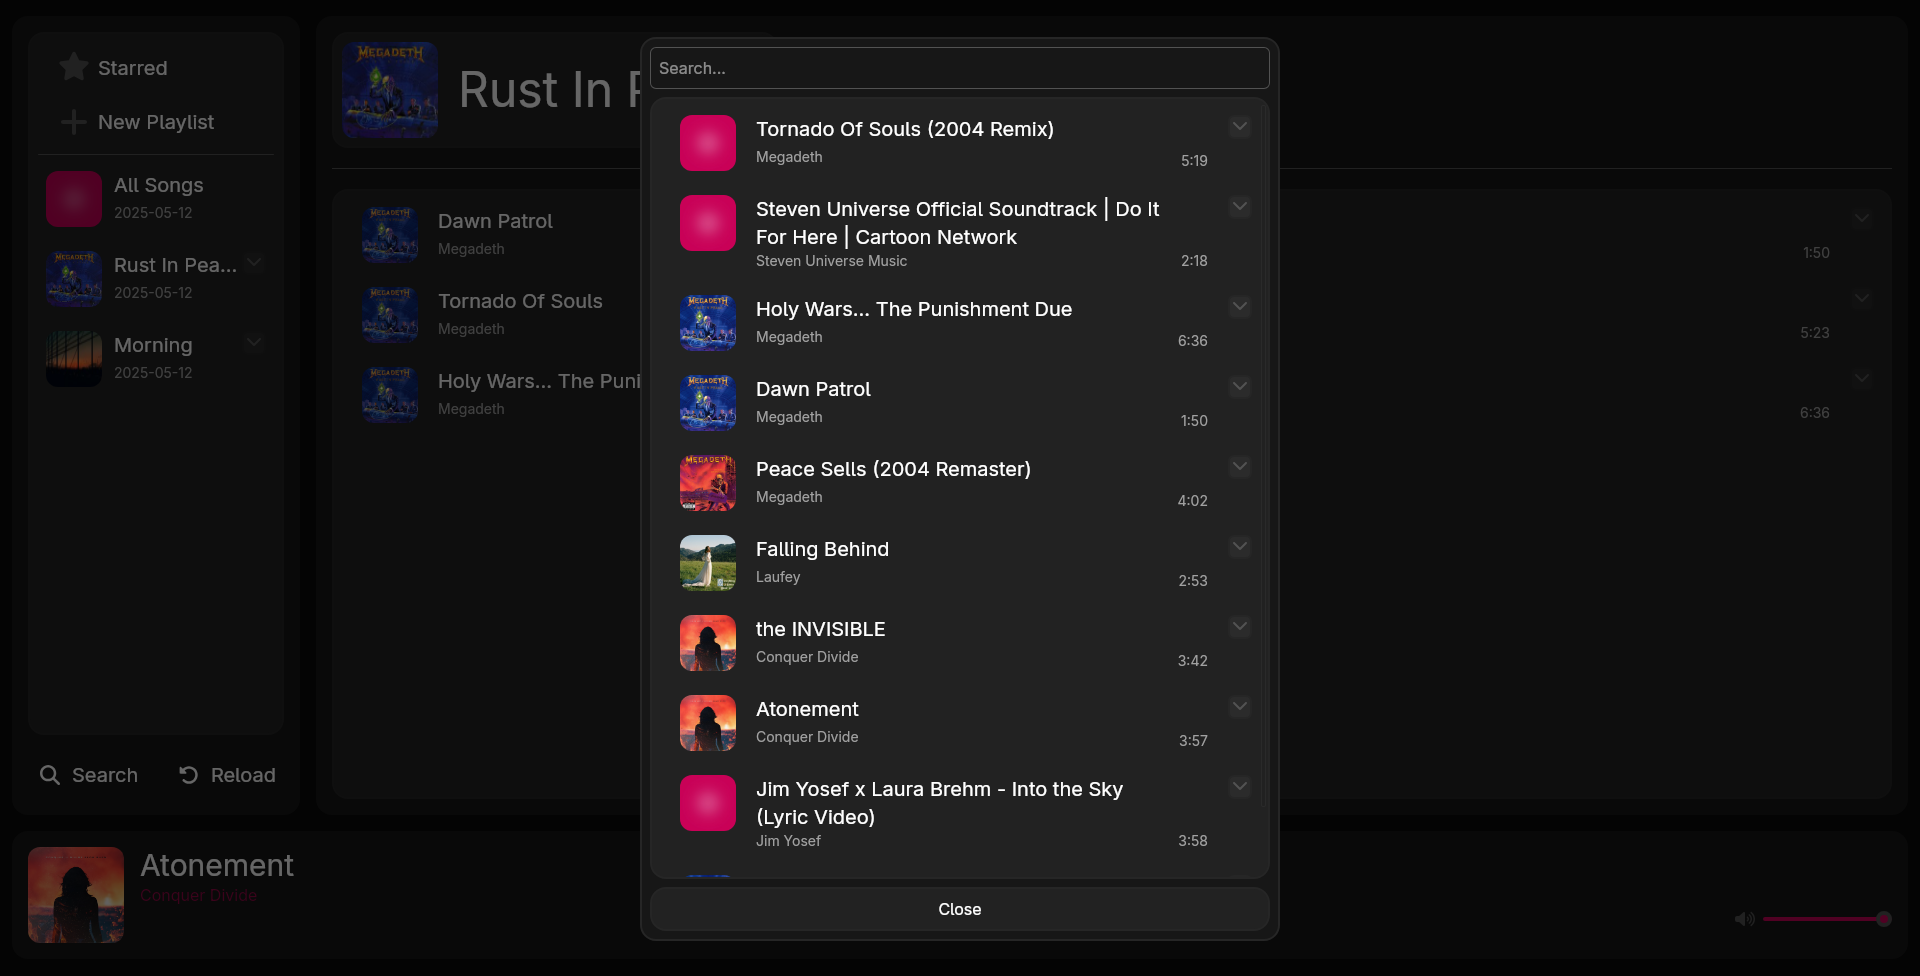
\includegraphics[width=0.8\textwidth]{media/screenshots/search_song.png}
                    \caption{Menú de buscar canción}
                    \label{fig:buscar}
                \end{figure}

                \begin{lstlisting}[caption={searchSong()}]
async searchSong() {
    await this.getAllSongs();
    this.filteredSongs = this.songs;
    this.isModalOpenSearch = true;
}

async getAllSongs() {
    const data_dir = await appDataDir();
    try {
      this.songs = await invoke<Song[]>('get_all_songs', {db_path: data_dir});
    } catch (error) {
      console.error('Error fetching songs:', error);
      this.songs = [];
    }
}
                \end{lstlisting}

                Cuando se activa la función de búsqueda mediante el botón correspondiente, se ejecuta el siguiente proceso: en primer lugar, se obtienen todas las canciones disponibles a través del método \verb|getAllSongs()|, que realiza una llamada al backend mediante Tauri IPC para recuperar los registros de la base de datos SQLite. Una vez completada esta operación, la lista completa de canciones se asigna a la variable \verb|filteredSongs| y se activa el modal de búsqueda estableciendo \verb|isModalOpenSearch| a \verb|true|. Este menú modal permite buscar y seleccionar canciones de toda la colección musical, ofreciendo las mismas capacidades de interacción que cuando las canciones se encuentran dentro de una playlist específica, funcionalidad que se detallará más adelante en la documentación.


            \subsubsection{Mainscreen}

            \begin{figure}[H]
                \centering
                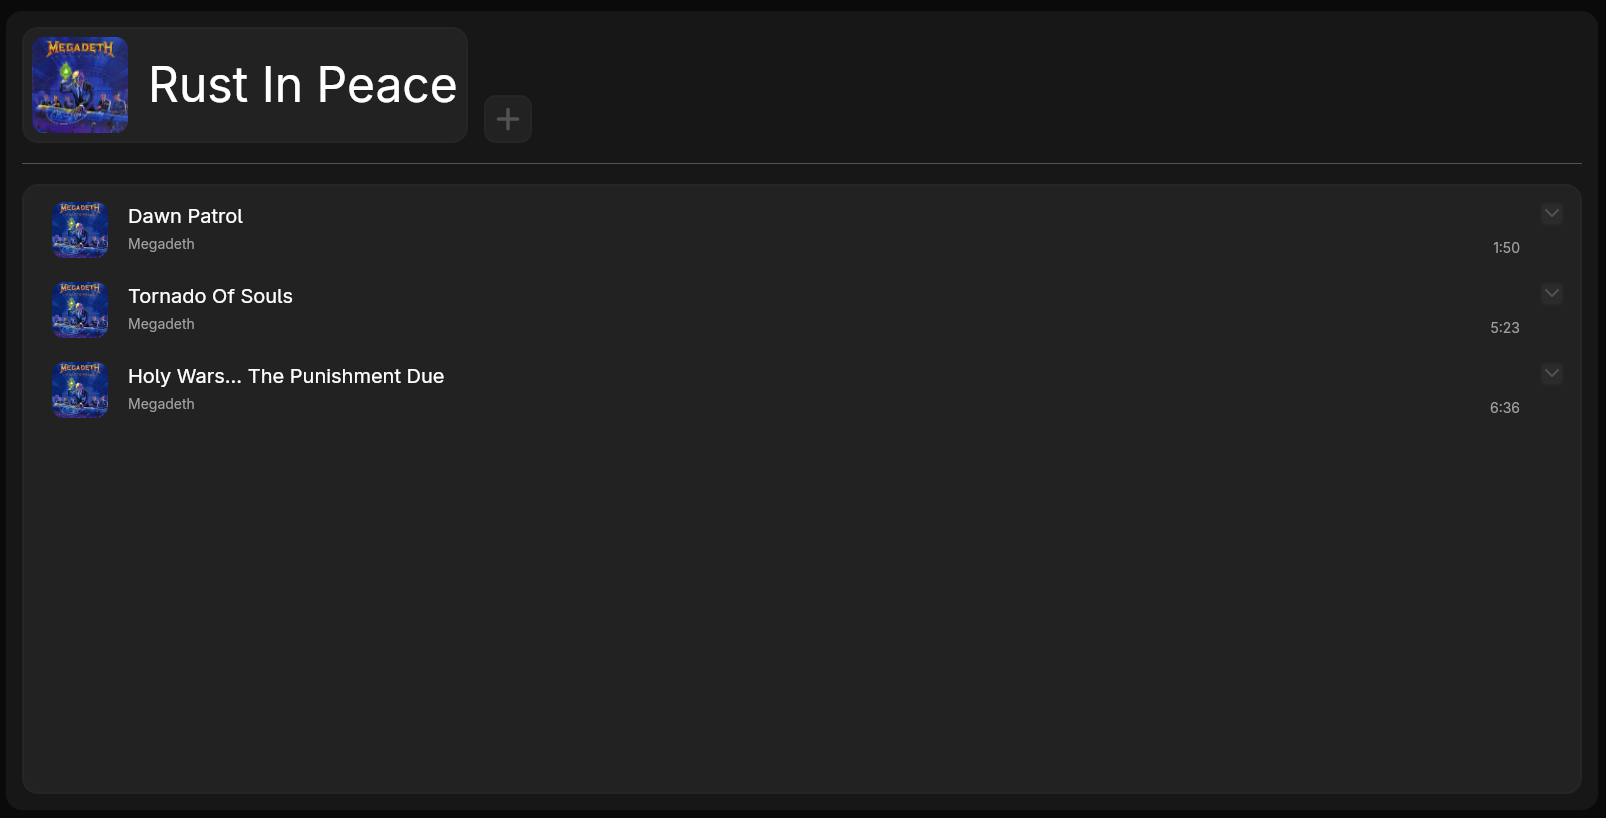
\includegraphics[width=1\textwidth]{media/screenshots/playlist.png}
                \caption{Mainscreen}
                \label{fig:Mainscreen}
            \end{figure}

            Este componente se encarga de mostrar la lista de canciones pertenecientes a una playlist, presentando para cada una:

            \begin{itemize}
                \item Información básica (título, artista, duración)
                \item Controles interactivos:
                \begin{itemize}
                    \item Botón de reproducción directa
                    \item Opción para añadir a la cola de reproducción
                \end{itemize}
            \end{itemize}

            La implementación de este componente sigue un principio de composición, donde la lógica sustancial se encuentra distribuida en sus subcomponentes especializados, mientras que el componente principal actúa principalmente como contenedor y coordinador de la visualización. \\

                \paragraph{Song Button}
                ‎

                \begin{figure}[H]
                    \centering
                    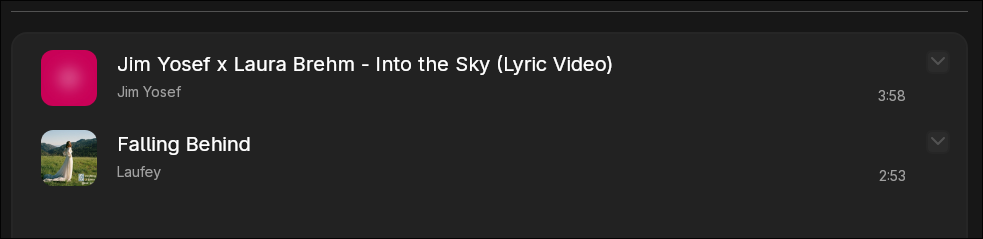
\includegraphics[width=1\textwidth]{media/screenshots/songbutton.png}
                    \caption{Song Button}
                    \label{fig:songbutton}
                \end{figure}

                Cada canción dentro de una playlist cuenta con un componente específico para su gestión y visualización de información. Al seleccionar el área principal del componente, se inicia automáticamente la reproducción del archivo de audio correspondiente. En la parte derecha del elemento se encuentra un menú desplegable (\textit{dropdown menu}) que proporciona las siguientes funcionalidades:

                \begin{itemize}
                    \item Añadir la canción a la cola de reproducción actual
                    \item Agregar la canción a otra playlist existente
                    \item Eliminar la canción de la playlist actual (función no disponible en la playlist \verb|All Songs|)
                \end{itemize}

                El concepto de \verb|All Songs|, que representa la colección completa de canciones disponibles, se explicará con mayor detalle en secciones posteriores de esta documentación.

                Los atributos del componente son:

                \begin{lstlisting}[caption={Atributos Song Button}]
isModalOpen: boolean = false;

isDropDownOpen: boolean = false;

constructor (public songManagement:SongManagementService, public songAdding:SongAddingService, public mainScreenStatus:MainScreenStatusService) {}

@Input() id!: string;
@Input() path!: string;
@Input() title!: string;
@Input() artist!: string;
@Input() album!: string;
@Input() year!: string;
@Input() duration!: string;
@Input() coverPath!: string;
@Input() isStarred!: boolean;

@Input() playlistId!: number;

coverUrl: string = 'assets/black.jpg';
                \end{lstlisting}

                Entre ellos se encuentran los metadatos de cada canción y la playlist en la que se encuentran mostrados ahora mismo. Estos datos son recibidos desde el componente padre. \\

                Además posee la interfaz \verb|Song|:

                \begin{lstlisting}[caption={Song}]
interface Song {
  id:string,
  path:string,
  title:string,
  artist:string,
  album:string,
  year:string,
  duration:string,
  coverPath:string,
  isStarred:boolean
}
                \end{lstlisting}

                El componente implementa diversos métodos para gestionar su funcionalidad, entre los cuales destaca:

                \begin{lstlisting}[caption={Dropdown menu}]
toggleDropDown() {
    this.isDropDownOpen = !this.isDropDownOpen;
}

closeDropDown() {
    this.isDropDownOpen = false;
}

@HostListener('document:click', ['$event'])
  onClickOutside(event: Event) {
    const target = event.target as HTMLElement;
    if (!target.closest('.relative.inline-block')) {
      this.closeDropDown();
    }
}
                \end{lstlisting}

                El menú desplegable (\textit{dropdown menu}) que contiene las opciones de gestión para cada canción implementa el siguiente comportamiento:

                \begin{itemize}
                    \item La visibilidad del menú se controla mediante el atributo booleano \verb|isDropDownOpen|
                    \item El método \verb|toggleDropDown()| alterna el estado de visibilidad
                    \item El método \verb|closeDropDown()| garantiza el cierre programático del menú
                \end{itemize}

                Para mejorar la experiencia de usuario, se implementa un cierre automático mediante el decorador \verb|@HostListener|, que detecta eventos de clic fuera del área del componente y ejecuta el cierre del menú cuando corresponde.

                \begin{lstlisting}[caption={playSong() y addSongToQueue()}]
playSong() {
    let song:Song = {id: this.id, path: this.path, title:this.title, artist: this.artist, album: this.album, year: this.year, duration: this.duration, coverPath: this.coverPath, isStarred: this.isStarred };
    this.songManagement.setOneSong(song);
}

addSongToQueue() {
    let song:Song = {id: this.id, path: this.path, title:this.title, artist: this.artist, album: this.album, year: this.year, duration: this.duration, coverPath: this.coverPath, isStarred: this.isStarred };
    this.songManagement.addOneSong(song);
}
                \end{lstlisting}

                Los métodos implementados siguen un patrón común donde los metadatos de la canción se estructuran en un objeto de tipo \verb|Song|, conteniendo todos los atributos relevantes (identificador, ruta, título, artista, álbum, año, duración, portada y estado de favorito). Este objeto se envía al servicio \verb|song-management|, diferenciándose en:

                \begin{itemize}
                    \item \verb|playSong()|: Inicia la reproducción inmediata mediante \verb|setOneSong()|
                    \item \verb|addSongToQueue()|: Añade la canción a la cola de reproducción usando \verb|addOneSong()|
                \end{itemize}

                \begin{lstlisting}[caption={addSongToPlaylist()}]
addSongToPlaylist() {
    this.songAdding.getAllPlaylists();
    this.isModalOpen = true;
}

close() {
    this.isModalOpen = false;
    this.songAdding.letGo();
}
                \end{lstlisting}

                El flujo de añadir canciones a playlists sigue un proceso estructurado:

                \begin{itemize}
                    \item \textbf{Fase de preparación}:
                    \begin{itemize}
                        \item Se obtienen todas las playlists disponibles mediante el servicio \verb|song-adding|.
                        \item Se activa el modal de selección estableciendo \verb|isModalOpen| a \verb|true|.
                    \end{itemize}
                    
                    \item \textbf{Fase de cierre}:
                    \begin{itemize}
                        \item Al completar la operación, se desactiva el modal (\verb|isModalOpen = false|).
                        \item Se liberan los recursos del servicio mediante \verb|letGo()| para optimizar memoria.
                    \end{itemize}
                \end{itemize}

                Este diseño garantiza una gestión eficiente de recursos durante el proceso de agregado de canciones a playlists.

                \begin{lstlisting}[caption={removeSongFromPlaylist()}]
async removeSongFromPlaylist() {
    const data_dir = await appDataDir();
    invoke('remove_song_from_playlist', {playlist_id: this.playlistId, song_id: this.id, db_path: data_dir});
    this.mainScreenStatus.refresh();
}
                \end{lstlisting}

                Cuando se activa la eliminación de una canción mediante el botón correspondiente, se ejecuta una petición al backend implementado en Rust que procesa la eliminación del registro en la base de datos SQLite. El método obtiene primero la ruta del directorio de datos mediante \verb|appDataDir()|, luego envía los parámetros necesarios (identificador de playlist, identificador de canción y ruta de la base de datos) a través de la función \verb|invoke()|. Finalmente, se actualiza el estado de la interfaz principal llamando al método \verb|refresh()| del servicio \verb|mainScreenStatus|, lo que garantiza que los cambios se reflejen inmediatamente en la vista del usuario.

                \begin{lstlisting}[caption={toggleStarred()}]
async toggleStarred() {
    const data_dir = await appDataDir();
    
    if (this.isStarred) {
      invoke('remove_is_starred', {song_id: this.id, db_path: data_dir});
      console.log("Canción !Starred: " + this.id);
    } else {
      invoke('add_is_starred', {song_id: this.id, db_path: data_dir});
      console.log("Canción Starred: " + this.id);
    }

    this.mainScreenStatus.refresh();
}
                \end{lstlisting}

                El método \verb|toggleStarred()| gestiona el estado de favorito de las canciones mediante un proceso que alterna entre dos posibles acciones. Cuando una canción está marcada como favorita (\verb|isStarred = true|), se ejecuta la función \verb|remove_is_starred| en el backend de Rust para eliminarla de la lista especial. En caso contrario, se invoca \verb|add_is_starred| para añadirla. En ambos casos, se utiliza \verb|appDataDir()| para obtener la ruta de la base de datos y se actualiza la interfaz mediante \\ \verb|mainScreenStatus.refresh()|. Las canciones marcadas como favoritas se agrupan automáticamente en una playlist especial accesible desde un botón específico en la barra lateral de la aplicación.

                \paragraph{Playlist Button}
                ‎

                Este componente de interfaz se activa exclusivamente cuando se inicia el menú modal para añadir canciones a playlists.

                Estos son sus atributos:

                \begin{lstlisting}[caption={Atributos Playlist Button}]
coverPath = 'assets/black.jpg';

constructor (public mainScreenStatus:MainScreenStatusService) {}

@Input() playlistId!: number;

@Input() playlistName!: string;

@Input() playlistCoverPath!: string;

@Input() songId!: string;
                \end{lstlisting}

                Su funcionamiento principal consiste en presentar al usuario la lista completa de playlists disponibles en el sistema, permitiendo la selección del destino donde se agregará la canción actual. \\

                Sus métodos más importantes son:

                \begin{lstlisting}[caption={getCoverPath()}]
async ngOnInit() {
    this.coverPath = await this.getCoverPath();
}

async getCoverPath(): Promise<string> {
    if (!this.coverPath) return 'assets/black.jpg';

    const fileData = await readFile(this.playlistCoverPath);

    const blob = new Blob([fileData], { type: 'image/jpeg' });

    if (this.coverPath) {
        URL.revokeObjectURL(this.coverPath);
    }

    return URL.createObjectURL(blob);
}
                \end{lstlisting}

                Este método, que sigue la misma implementación ya descrita en el componente anterior, se encarga de gestionar la visualización de las portadas de las playlists.

                \begin{lstlisting}[caption={addSongToPlaylist()}]
async addSongToPlaylist() {
    const data_dir = await appDataDir();
    invoke('add_song_to_playlist', {playlist_id: this.playlistId, song_id: this.songId, db_path: data_dir})
    this.mainScreenStatus.refresh();
}
                \end{lstlisting}

                El método \verb|addSongToPlaylist()| ejecuta el proceso de añadir una canción a una playlist específica mediante una llamada al backend implementado en Rust. Primero obtiene el directorio de datos de la aplicación usando \verb|appDataDir()|, luego envía los parámetros necesarios (ID de la playlist, ID de la canción y ruta de la base de datos) a través de la función \verb|invoke()|. Finalmente, actualiza la página principal llamando a \verb|mainScreenStatus.refresh()| para reflejar los cambios en la interfaz de usuario. Este flujo garantiza que la canción quede registrada en la base de datos y que la vista se actualice consistentemente.

                \paragraph{Homeitem}
                ‎

                El componente \verb|Homeitem| representa una implementación alternativa al componente estándar \verb|Song|, desarrollado específicamente para cumplir con requerimientos particulares de diseño y funcionalidad en la playlist \textit{Starred Songs}.

            \subsubsection{Servicios}

            Se han implementado servicios especializados para cada funcionalidad clave, tales como el manejo de listas de reproducción, la gestión de metadatos musicales y la información de la \verb|mainscreen|.

                \paragraph{Main Screen Status}
                ‎

                \begin{lstlisting}[caption={Atributos Main Screen Status}]
onHome = signal(true);
pId: number = 0;
pName: string = "";
pDate: string = "";
pCoverPath: string = "";
pStarred: boolean = false;

songs:Song[] = []

constructor(public songManagement:SongManagementService) { }
                \end{lstlisting}

                El servicio \verb|MainScreenStatus| se encarga de gestionar y mantener el estado de la información mostrada en la interfaz principal de la aplicación (\verb|mainscreen|). Para ello, se han definido una serie de atributos que almacenan tanto los metadatos de la playlist actualmente visualizada como las canciones asociadas a la misma.

                Entre los atributos principales se incluyen señales y variables que controlan el estado de la interfaz (\verb|onHome|), así como información específica de la playlist, como su identificador (\verb|pId|), nombre (\verb|pName|), fecha de creación (\verb|pDate|), ruta de la portada (\verb|pCoverPath|) y estado de favorito (\verb|pStarred|). Adicionalmente, se almacena un arreglo de canciones (\verb|songs|) que pertenecen a la playlist actual. Por supuesto este servicio contiene la interfaz \verb|Song| vista anteriormente.

                El servicio se inicializa con una dependencia inyectada del \\ \verb|SongManagementService|, lo que permite una coordinación fluida entre la gestión del estado de la interfaz y las operaciones relacionadas con la reproducción de audio. Esta arquitectura modular facilita el mantenimiento y la escalabilidad del código. \\


                \begin{lstlisting}[caption={setHome() y setPlaylist()}]
setHome() {
    this.onHome.set(true);
    this.pId = 0;
    this.pName = "";
    this.pDate = "";
    this.pCoverPath = "";
    this.getAllStarred();
}

setPlaylist(id:number, name:string, date:string, coverPath:string, isStarred:boolean) {
    this.onHome.set(false);
    this.pId = id;
    this.pName = name;
    this.pDate = date;
    this.pCoverPath = coverPath;
    this.pStarred = isStarred;
}
                \end{lstlisting}

                Los métodos \verb|setHome()| y \verb|setPlaylist()| gestionan la transición entre las diferentes vistas de la interfaz principal (\verb|mainscreen|). En el primer caso, \verb|setHome()| configura el estado para mostrar la lista de canciones marcadas como favoritas, estableciendo el valor \verb|onHome| a \verb|true| y reiniciando los metadatos de la playlist. Simultáneamente, se invoca el método \verb|getAllStarred()| para cargar las canciones destacadas.

                Por otro lado, \verb|setPlaylist()| se utiliza para visualizar una playlist específica, actualizando los metadatos correspondientes (\verb|id|, \verb|name|, \verb|date|, \verb|coverPath| y estado \verb|isStarred|) y desactivando la vista de favoritos mediante \verb|onHome.set(false)|.

                Cabe destacar que la nomenclatura original (\verb|Home|) fue heredada de las primeras etapas del desarrollo, cuando la estructura conceptual del proyecto aún estaba en definición. Posteriormente, esta terminología se actualizó a \verb|Starred Songs| para reflejar con mayor precisión su funcionalidad. A pesar de este cambio, se mantuvieron las referencias originales en el código para preservar la compatibilidad con los componentes existentes.

                Se ha considerado una refactorización futura para unificar la nomenclatura y mejorar la coherencia del código. Actualmente, aunque los términos \verb|Home| y \verb|Starred Songs| coexisten, esta dualidad no afecta la funcionalidad del sistema. \\

                \begin{lstlisting}[caption={Obtención de playlists}]
async getAllSongs() {
    const data_dir = await appDataDir();
    try {
      this.songs = await invoke<Song[]>('get_all_songs', {db_path: data_dir});
    } catch (error) {
      console.error('Error fetching songs:', error);
      this.songs = [];
    }
}

async getAllStarred() {
    const data_dir = await appDataDir();
    try {
      this.songs = await invoke<Song[]>('get_all_starred', {db_path: data_dir});
    } catch (error) {
      console.error('Error fetching songs:', error);
      this.songs = [];
    }
}

async getPlaylistSongs() {
    const data_dir = await appDataDir();
    try {
      this.songs = await invoke<Song[]>('get_playlist_songs', {playlist_id: this.pId, db_path: data_dir});
    } catch (error) {
      console.error('Error fetching songs:', error);
      this.songs = [];
    }
}
                \end{lstlisting}

                Los métodos \verb|getAllSongs()|, \verb|getAllStarred()| y \verb|getPlaylistSongs()| gestionan la obtención de canciones desde diferentes fuentes, asignándolas posteriormente a la variable local \verb|songs|. En cada caso, se sigue un patrón similar: primero se obtiene el directorio de datos de la aplicación mediante \verb|appDataDir()|, luego se realiza una llamada al backend mediante \verb|invoke()|, y finalmente se manejan tanto el éxito como los posibles errores de la operación.

                \begin{lstlisting}[caption={refresh()}]
async refresh() {
    if (this.pId != 0) {
      await this.getPlaylistSongs();
    } else if (this.pId == 0 && this.onHome()) {
      await this.getAllStarred();
    } else {
      await this.getAllSongs();
    }
}
                \end{lstlisting}

                El método \verb|refresh()| se encarga de actualizar dinámicamente el contenido mostrado en la \verb|mainscreen| en función del contexto actual de reproducción. Para ello, se implementa un flujo condicional que evalúa el identificador de playlist almacenado en \verb|this.pId| y el estado de la señal \verb|onHome|.

                Este enfoque garantiza que la interfaz siempre muestre el contenido más relevante según el estado actual de la aplicación, manteniendo una experiencia de usuario coherente. La implementación mediante llamadas asíncronas (\verb|await|) asegura que las operaciones de actualización se completen antes de proceder con cualquier otra acción, evitando así condiciones de carrera o estados inconsistentes en la interfaz.

                \begin{lstlisting}[caption={playQueue() y addQueue()}]
playQueue() {
    this.songManagement.setQueue(this.songs);
  }

addQueue() {
    this.songManagement.addQueue(this.songs);
}
                \end{lstlisting}

                Estos métodos gestionan la interacción con la cola de reproducción a través del servicio \verb|SongManagementService|. Al pulsar sobre el nombre de la playlist, se invoca \verb|playQueue()|, que establece la lista actual de canciones (\verb|this.songs|) como nueva cola de reproducción mediante el método \verb|setQueue()| del servicio. De forma similar, al seleccionar la opción de añadir a cola, \verb|addQueue()| incorpora las canciones a la cola existente utilizando \verb|addQueue()| del mismo servicio.

                Esta implementación refleja una arquitectura limpia donde la lógica de gestión de reproducción se delega completamente al servicio, permitiendo que los componentes se centren únicamente en la presentación de datos y captura de eventos de usuario. El servicio \\ \verb|SongManagementService| será analizado en profundidad en la siguiente sección de esta documentación.

                \paragraph{Song Management}
                ‎

                \begin{lstlisting}[caption={Atributos Song Management}]
songCover:string = ""
songTitle:string = ""
songArtist:string = ""

constructor() { this.setupSongListeners() }

song: HTMLAudioElement = new Audio();

volume:number = 0;

isPlaying:boolean = false;

loopMode:string = "none" //* none - playlist - single
shuffle:boolean = false

queue:Song[] = []
queueSave:Song[] = []
currentIndex:number = 0
currentIndexSave:number = 0
currentISDelay:number = 0

progress:number = 0;
                \end{lstlisting}

                El servicio \verb|SongManagementService| centraliza toda la lógica relacionada con la reproducción musical y gestión de colas en la aplicación. Sus atributos principales pueden categorizarse en tres grupos:

                \begin{enumerate}
                    \item \textbf{Metadatos visuales}: Almacena información de la canción actual (\verb|songCover|, \verb|songTitle|, \verb|songArtist|) para mostrarse en la interfaz.
                    \item \textbf{Control de reproducción}: Incluye el elemento \verb|HTMLAudioElement| para manejo nativo del audio, junto con estados como \verb|isPlaying|, \verb|volume| y \verb|progress| que reflejan la reproducción en tiempo real.
                    \item \textbf{Gestión de cola}: Mantiene dos versiones de la cola (\verb|queue| y \verb|queueSave|) para implementar funcionalidades como shuffle, junto con índices de posición (\verb|currentIndex|, \verb|currentIndexSave|) y modos especiales (\verb|loopMode|, \verb|shuffle|).
                \end{enumerate}

                El constructor inicializa automáticamente los listeners de eventos mediante \verb|setupSongListeners()|, preparando el servicio para responder a cambios de estado.

                \begin{lstlisting}[caption={setUpSongListeners()}]
private async setupSongListeners() {
    this.song?.addEventListener('ended', () => this.playNext());
    this.song?.addEventListener('timeupdate', () => {
      if (this.song) {
        this.progress = (this.song.currentTime / this.song.duration) * 100;
      }
    });
}
                \end{lstlisting}

                El método \verb|setupSongListeners()| configura los listeners esenciales para el control de reproducción, implementando dos funcionalidades clave mediante eventos sobre el elemento \verb|HTMLAudioElement|.
                
                \begin{enumerate}
                    \item El evento 'ended' activa automáticamente \verb|playNext()| al terminar la canción actual, permitiendo una reproducción continua.
                    \item Segundo, el evento 'timeupdate' actualiza constantemente la propiedad \verb|progress| con el porcentaje de avance (calculado como la relación entre \verb|currentTime| y \verb|duration|), lo que se refleja en la barra de progreso de la interfaz.
                \end{enumerate}

                \begin{lstlisting}[caption={getCoverPath()}]
async getCoverPath(coverPath:string): Promise<string> {
    let coverUrl: string = 'assets/black.jpg';
    if (!coverPath) return coverUrl;

    const fileData = await readFile(coverPath);
    
    const blob = new Blob([fileData], { type: 'image/jpeg' });

    if (coverUrl) {
      URL.revokeObjectURL(coverUrl);
    }

    return URL.createObjectURL(blob);

}
                \end{lstlisting}

                El método \verb|getCoverPath()| representa una solución centralizada para la gestión de portadas de las canciones, cuya implementación fue migrada desde el componente \verb|playbar| al servicio actual como parte de una refactorización para simplificar la arquitectura. Esta implementación unificada elimina la duplicación de código que existía cuando la funcionalidad estaba dispersa en varios componentes (a excepción de las playlists), mejorando el mantenimiento y permitiendo una gestión más eficiente de los recursos multimedia.

                \begin{lstlisting}[caption={loadAndPlay()}]
async loadAndPlay(_path:string, _index:number) {
    try {
      this.songTitle = this.queue[_index].title;
      this.songArtist = this.queue[_index].artist;
      
      this.songCover = await this.getCoverPath(this.queue[_index].coverPath);

      const path = _path;
      
      const fileData = await readFile(path);
      const blob = new Blob([fileData], { type: 'audio/mp3' });
      const audioUrl = URL.createObjectURL(blob);
      
      this.song.src = audioUrl;
      await this.song.play();
      this.isPlaying = true;
      
      console.log('Canción cargada correctamente');
    } catch (error) {
      console.error('Error al cargar la canción:', error);
    }
}
                \end{lstlisting}

                El método \verb|loadAndPlay()| gestiona todo el proceso de preparación y reproducción de canciones mediante un flujo secuencial. Primero actualiza los metadatos visuales (\verb|songTitle|, \verb|songArtist| y \verb|songCover|) utilizando los datos de la canción en la posición \verb|_index| de la cola. Para la portada, se emplea el método \verb|getCoverPath()| previamente descrito. Luego carga el archivo de audio desde la ruta especificada (\verb|_path|), lo convierte a un blob y genera una URL temporal para su reproducción. Finalmente asigna esta URL al elemento de audio (\verb|this.song.src|) e inicia la reproducción, actualizando el estado \verb|isPlaying|. Todo el proceso está encapsulado en un bloque try-catch que maneja posibles errores durante la carga.

                \begin{lstlisting}[caption={set y add}]
setQueue(songs:Song[]) {
    this.queue = [...songs];
    this.currentIndex = 0;
    this.loadAndPlay(this.queue[0].path, 0);
}

addQueue(songs: Song[]) {
    this.queue.push(...songs)
}

setOneSong(song:Song) {
    this.queue = [];
    this.queue.push(song);
    this.currentIndex = 0;
    this.loadAndPlay(this.queue[0].path, 0);
}

addOneSong(song:Song) {
    this.queue.push(song);
}
                \end{lstlisting}

                Estos métodos constituyen la API fundamental para la gestión de la cola de reproducción, mencionada recurrentemente en secciones anteriores de la documentación. La implementación sigue un patrón dual con variantes "set" (establecer) y "add" (añadir):

                Los métodos \verb|setQueue()| y \verb|setOneSong()| reemplazan completamente la cola existente. En el primer caso, se recibe un array de canciones que se copia mediante el operador de propagación (\verb|...songs|), mientras que el segundo acepta una única canción, reiniciando la cola antes de añadirla. Ambos métodos comparten el mismo flujo posterior: reinician el índice actual a 0 e invocan \verb|loadAndPlay()| para comenzar la reproducción inmediata.

                Por otro lado, \verb|addQueue()| y \verb|addOneSong()| implementan la funcionalidad complementaria de añadir contenido a la cola existente sin modificar el estado de reproducción actual. La versión \verb|addQueue()| utiliza el mismo operador de propagación para incorporar múltiples canciones, mientras que \verb|addOneSong()| trabaja con elementos individuales.

                \begin{lstlisting}[caption={togglePlayPause()}]
async togglePlayPause() {
    if(!this.isPlaying) {
      this.song.play()
    } else {
      this.song.pause()
    }
    this.isPlaying = !this.isPlaying;
}
                \end{lstlisting}
                 
                El método \verb|togglePlayPause()| implementa la funcionalidad básica de control de reproducción mediante un mecanismo de alternancia. Cuando se invoca, verifica el estado actual de reproducción a través de la variable \verb|isPlaying|. Si la reproducción está pausada (\verb|isPlaying| es falso), se ejecuta el método \verb|play()| del elemento de audio HTML. En caso contrario, se activa el método \verb|pause()|. Finalmente, se invierte el valor de \verb|isPlaying| para reflejar el nuevo estado.

                \begin{lstlisting}[caption={playNext() y playPrevious()}]
playNext() {
    if ((this.currentIndex < this.queue.length - 1) && (this.loopMode == "none" || this.loopMode == "playlist")) {
      this.currentIndex++;
      this.currentISDelay++;
      this.loadAndPlay(this.queue[this.currentIndex].path, this.currentIndex);
    } else if ((this.currentIndex == this.queue.length - 1) && this.loopMode == "playlist") {
      this.currentIndex = 0;
      this.loadAndPlay(this.queue[this.currentIndex].path, this.currentIndex);
    } else if (this.loopMode == "single") {
      this.song.currentTime = 0
    } else {
      this.stop();
    }
    console.log("CurrentIndex: " + this.currentIndex + " CurrentIndexSave: " + this.currentIndexSave)
}

playPrevious() {
    if(this.song.currentTime < 3) {
      if((this.currentIndex > 0) && this.loopMode != "single") {
        this.currentIndex--;
        this.currentISDelay--;
        this.loadAndPlay(this.queue[this.currentIndex].path, this.currentIndex);
      } else if (this.currentIndex == 0) {
        if (this.loopMode == "playlist") {
          this.currentIndex = this.queue.length - 1
          this.loadAndPlay(this.queue[this.currentIndex].path, this.currentIndex);
        } else if(this.loopMode == "single") {
          this.song.currentTime = 0
        } else {
          this.stop()
        }
      } else {
        this.song.currentTime = 0
      }
    } else {
      this.song.currentTime = 0
    }
    
}

stop() {
    this.song.pause();
    this.song.currentTime = 0;
    this.isPlaying = false;
}
                \end{lstlisting}

                Estos métodos implementan la lógica avanzada de navegación en la cola de reproducción, considerando diferentes modos de funcionamiento (\verb|none|, \verb|playlist| y \verb|single|). En \verb|playNext()|, se evalúa primero si hay canciones siguientes disponibles y el modo de repetición lo permite, incrementando entonces el índice y cargando la siguiente canción. Cuando se alcanza el final de la lista en modo \verb|playlist|, se reinicia al principio. Para el modo \verb|single|, simplemente se reinicia la canción actual.

                El método \verb|playPrevious()| incorpora lógica adicional para diferenciar entre retroceder a la canción anterior (si la reproducción actual lleva menos de 3 segundos) o reiniciar la canción actual. Maneja correctamente los casos especiales como el inicio de la lista en modo \verb|playlist| (saltando al final) o el comportamiento específico del modo \verb|single|. Ambos métodos mantienen actualizados los índices de posición (\verb|currentIndex|, \verb|currentISDelay|) y registran el estado actual para depuración.

                La implementación demuestra un manejo robusto de todos los casos posibles de navegación, proporcionando una experiencia de usuario consistente con los reproductores musicales profesionales. El diseño modular permite fácil extensión para añadir nuevos modos de reproducción o comportamientos especiales en futuras iteraciones.

                \begin{lstlisting}[caption={Control de tiempo y volumen}]
onInput(event: Event) {
    const input = event.target as HTMLInputElement;
    const newTime = parseInt(input.value);
    if (this.song) {
      this.song.currentTime = newTime;
    }
}

onVolume(event: Event) {
    const inputVolume = event.target as HTMLInputElement;
    const newVolume = parseInt(inputVolume.value) / 100;
    if (this.song) {
      this.song.volume = newVolume;
    }
    this.volume = parseInt(inputVolume.value);
    return this.volume
}
                \end{lstlisting}

                Estos métodos gestionan la interacción del usuario con los controles de reproducción. El método \verb|onInput()| se encarga de actualizar la posición de reproducción cuando el usuario manipula la barra de progreso. Primero obtiene el valor del elemento HTML que generó el evento, lo convierte a número entero y luego actualiza la propiedad \verb|currentTime| del elemento de audio si este está disponible.

                Por su parte, \verb|onVolume()| controla los ajustes de volumen mediante un flujo similar: captura el valor del control deslizante de volumen, lo normaliza dividiendo entre 100 (para adaptarlo al rango 0-1 que espera el API de audio) y aplica este valor tanto al elemento de audio como a la variable local \verb|volume|. La conversión de tipos y normalización de valores garantiza que los controles funcionen consistentemente aunque provengan de diferentes fuentes de entrada.

                Ambos métodos implementan una verificación de existencia (\verb|if (this.song)|) como medida de seguridad para evitar errores cuando no hay elemento de audio inicializado.

                \begin{lstlisting}[caption={cycleLoop()}]
cycleLoop() {
    switch (this.loopMode) {
      case "none":
        this.loopMode = "playlist";
        break;
      case "playlist":
        this.loopMode = "single";
        break;
      case "single":
        this.loopMode = "none";
        break;
      default:
        this.loopMode = "none";
        break;
    }
    return this.loopMode;
}
                \end{lstlisting}

                Este método se encarga de alternar cíclicamente la variable \verb|loopMode|.

                \begin{lstlisting}[caption={Shuffle}]
toggleShuffle() {
    if(!this.shuffle) {
      this.queueSave = [...this.queue];
      this.currentIndexSave = this.currentIndex;
      this.doShuffle();
    } else if(this.shuffle) {
      this.currentIndex = this.queueSave.indexOf(this.queue[this.currentIndex]);
      this.queue = this.queueSave;
    }
    this.shuffle = !this.shuffle;
    return this.shuffle;
  }

doShuffle() {
    this.queue.unshift(this.queue[this.currentIndex])
    this.queue.splice(this.currentIndex+1,1)
    this.currentIndex = 0
    let firstElement = this.queue[0]
    let queueToShuffle = this.queue.splice(1);
    let currentIndex2 = queueToShuffle.length;

    while (currentIndex2 != 0) {

      let randomIndex = Math.floor(Math.random() * currentIndex2);
      currentIndex2--;

      [queueToShuffle[currentIndex2], queueToShuffle[randomIndex]] = [queueToShuffle[randomIndex], queueToShuffle[currentIndex2]];
    }
    queueToShuffle.unshift(firstElement)
    this.queue = queueToShuffle
    
}
                \end{lstlisting}

                La implementación del modo aleatorio (\textit{shuffle}) sigue un enfoque de dos fases mediante los métodos \verb|toggleShuffle()| y \verb|doShuffle()|. Cuando se activa el modo aleatorio, \verb|toggleShuffle()| preserva el estado original de la cola (\verb|queueSave|) y la posición actual (\verb|currentIndexSave|) antes de aplicar la aleatorización. Este diseño permite restaurar el orden inicial cuando se desactiva la función, manteniendo la coherencia con el comportamiento de reproductores profesionales.

                El método \verb|doShuffle()| implementa el algoritmo Fisher-Yates (\textcite{wikifisheryates}) para la mezcla aleatoria, optimizado para garantizar que la canción actual permanezca en primera posición durante la transición. El proceso consta de tres etapas: \begin{enumerate}
                  \item Extracción y protección de la canción en reproducción.
                  \item Mezcla aleatoria del resto de la cola mediante intercambios indexados.
                  \item reconstrucción de la cola con la canción actual preservada.
                \end{enumerate}
                
                Esta implementación demuestra especial atención al detalle en la experiencia de usuario, evitando saltos bruscos en la reproducción durante la activación del modo aleatorio.

                El sistema mantiene sincronizados los estados paralelos (colas original y aleatoria, índices de posición) mediante operaciones atómicas, garantizando consistencia incluso en listas extensas. La solución combina eficiencia computacional (complejidad O(n) para la mezcla) con un diseño intuitivo que refleja los patrones de uso establecidos en aplicaciones de referencia del sector.

                \begin{lstlisting}[caption={formatTime()}]
formatTime(seconds: number | undefined): string {
    if (seconds === undefined || isNaN(seconds)) return '0:00';
    
    const minutes = Math.floor(seconds / 60);
    const remainingSeconds = Math.floor(seconds % 60);
    
    const paddedSeconds = remainingSeconds.toString().padStart(2, '0');
    
    return `${minutes}:${paddedSeconds}`;
}
                \end{lstlisting}

                El método \verb|formatTime()| implementa la conversión de segundos a un formato de tiempo legible (MM:SS) para la interfaz de usuario. Cuando recibe un valor indefinido o no numérico, devuelve por defecto '0:00' para mantener la consistencia visual. Para valores válidos, realiza tres operaciones matemáticas: primero calcula los minutos completos mediante división entera, luego obtiene los segundos restantes usando el operador módulo, y finalmente aplica un padding de dos dígitos a los segundos para mantener un formato uniforme.

                La salida cumple con los estándares de reproductores musicales profesionales, mostrando siempre minutos y segundos con dos dígitos (ej: 3:05 en lugar de 3:5), lo que mejora la legibilidad y experiencia de usuario durante la reproducción.

                \paragraph{Song Adding}
                ‎

                El servicio \verb|SongAddingService| se especializa en la gestión de playlists durante el proceso de añadir canciones. Su diseño minimalista cumple con el principio de responsabilidad única, enfocándose exclusivamente en dos operaciones clave: la obtención de playlists y la liberación de recursos.

                \begin{lstlisting}[caption={song-adding.service.ts}]
export class SongAddingService {
  playlists: Playlist[] = []

  constructor() { }

  async getAllPlaylists() {
    const data_dir = await appDataDir();
    try {
      this.playlists = await invoke<Playlist[]>('get_all_playlists', {db_path: data_dir});
    } catch (error) {
      console.error('Error fetching playlists:', error);
      this.playlists = [];
    }
  }


  letGo() {
    this.playlists = [];
  }


}

interface Playlist {
  id: number;
  name: string;
  creation_date: string;
  cover_path: string;
  isStarred: boolean;
}
                \end{lstlisting}

                El método principal \verb|getAllPlaylists()| establece comunicación con el backend mediante Tauri (\verb|invoke|), recuperando el listado completo de playlists desde la base de datos SQLite, este listado es mapeado en la parte de HTML del componente \textit{Song}. Implementa manejo de errores robusto que garantiza estabilidad incluso ante fallos de conexión, inicializando un array vacío como fallback. La interfaz \verb|Playlist| define la estructura de datos esperada, incluyendo metadatos esenciales como identificador único, nombre, fecha de creación, ruta de la portada y estado de favorito.

                La función \verb|letGo()| proporciona un mecanismo de limpieza de memoria, liberando el array de playlists cuando ya no es necesario. Este enfoque refleja buenas prácticas de gestión de recursos en aplicaciones con componentes modales, donde la memoria puede acumularse durante ciclos repetidos de apertura/cierre.

        \subsection{Backend}

        Rust y SQLite

            \subsubsection{Tauri API}

            El archivo \verb|lib.rs| constituye el punto de entrada principal del backend desarrollado con Tauri y Rust, donde se configura la aplicación y se definen los manejadores de las operaciones entre el frontend y el sistema. Su estructura sigue un flujo bien definido que combina inicialización de plugins, gestión de permisos y registro de comandos invocables.

            \begin{lstlisting}[caption={lib.rs}]
use std::path::PathBuf;
use logic::add_playlist;
use logic::add_song;
use logic::add_starred;
use logic::remove_song;
use logic::remove_a_playlist;
use logic::remove_starred;
use tauri_plugin_fs::FsExt;

mod logic;
use logic::Playlist;
use logic::Song;

#[tauri::command(rename_all = "snake_case")]
async fn sync_lib(music_dir:String, app_data_dir:String) {
    let _ = logic::sync(PathBuf::from(app_data_dir),PathBuf::from(music_dir));
}


#[tauri::command(rename_all = "snake_case")]
async fn get_all_playlists(db_path:String) -> Result<Vec<Playlist>, String> {
    let playlists = logic::get_all_playlists(db_path)?;

    Ok(playlists)
}

#[tauri::command(rename_all = "snake_case")]
async fn get_all_songs(db_path:String) -> Result<Vec<Song>, String> {
    let all_songs = logic::get_all_songs(db_path)?;

    Ok(all_songs)
}

#[tauri::command(rename_all = "snake_case")]
async fn get_playlist_songs(playlist_id: i64, db_path: String) -> Result<Vec<Song>, String> {
    let playlist_songs = logic::get_playlist_songs(playlist_id, db_path)?;

    Ok(playlist_songs)
}

#[tauri::command(rename_all = "snake_case")]
async fn get_all_starred(db_path:String) -> Result<Vec<Song>, String> {
    let all_songs = logic::get_all_songs_starred(db_path)?;

    Ok(all_songs)
}

#[tauri::command(rename_all = "snake_case")]
async fn create_playlist(name:String, cover_path:String, db_path:String) {
    let _ = add_playlist(name, cover_path, db_path);
}

#[tauri::command(rename_all = "snake_case")]
async fn remove_playlist(playlist_id:i64, db_path:String) {
    let _ = remove_a_playlist(playlist_id, db_path);
}

#[tauri::command(rename_all = "snake_case")]
async fn add_song_to_playlist(playlist_id:i64, song_id:String, db_path:String) {
    let _ = add_song(playlist_id, song_id, db_path);
}

#[tauri::command(rename_all = "snake_case")]
async fn remove_song_from_playlist(playlist_id:i64, song_id:String, db_path:String) {
    let _ = remove_song(playlist_id, song_id, db_path);
}

#[tauri::command(rename_all = "snake_case")]
async fn add_is_starred(song_id:String, db_path:String) {
    let _ = add_starred(song_id, db_path);
}

#[tauri::command(rename_all = "snake_case")]
async fn remove_is_starred(song_id:String, db_path:String) {
    let _ = remove_starred(song_id, db_path);
}

#[cfg_attr(mobile, tauri::mobile_entry_point)]
pub fn run() {
    tauri::Builder::default()
        .plugin(tauri_plugin_opener::init())
        .plugin(tauri_plugin_dialog::init())
        .plugin(tauri_plugin_fs::init())
        .setup(|app| {
            let scope = app.fs_scope();
            if let Err(e) = scope.allow_directory("$HOME/Music", true) {
                eprintln!("Failed access: {}", e)
            }
            if let Err(e) = scope.allow_directory("$APPDATA", true) {
                eprintln!("Failed access: {}", e)
            }
            if let Err(e) = scope.allow_directory("$HOME/.config", true) {
                eprintln!("Failed access: {}", e)
            }
            if let Err(e) = scope.allow_directory("$HOME/Library/Application Support", true) {
                eprintln!("Failed access: {}", e)
            }
            if let Err(e) = scope.allow_directory("src-tauri", true) {
                eprintln!("Failed access: {}", e)
            }
            
            Ok(())
         })
        .invoke_handler(tauri::generate_handler![sync_lib, get_all_playlists, get_all_songs, get_playlist_songs, get_all_starred,create_playlist, remove_playlist, add_song_to_playlist, remove_song_from_playlist, add_is_starred, remove_is_starred])
        .run(tauri::generate_context!())
        .expect("error while running tauri application");
}
              
            \end{lstlisting}
            
            En la fase de setup, se definen los directorios accesibles para la aplicación mediante \verb|fs_scope()|, abarcando ubicaciones críticas multiplataforma:

            \begin{itemize}
              \item Directorios de música (\$HOME/Music).
              \item Rutas de configuración según el SO (\verb|$APPDATA| en Windows, \verb|$HOME/.local/share/| en Linux, \verb|Library/Application Support| en macOS).
            \end{itemize}

            El método \verb|invoke_handler| asocia las funciones Rust con llamadas desde el frontend mediante \verb|generate_handler!|.

            Los handlers registrados incluyen:

            \begin{itemize}
              \item Gestión de playlists (\verb|create_playlist|, \verb|remove_playlist|)
              \item Consultas a la base de datos (\verb|get_all_songs|)
              \item Control de canciones destacadas (\verb|add_is_starred|)
            \end{itemize}

            Finalmente, el builder se ejecuta con \verb|run()|, propagando cualquier error durante el arranque.

            \subsubsection{Diseño de la base de datos}

            \begin{figure}[H]
              \centering
              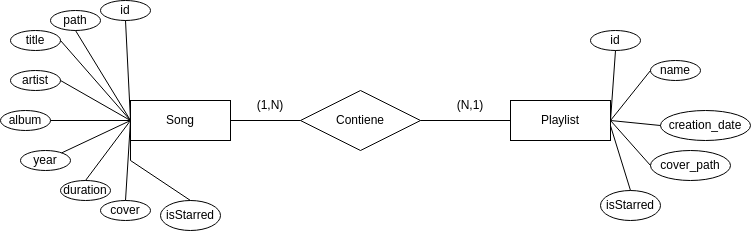
\includegraphics[width=0.8\textwidth]{media/ER.drawio.png}
              \caption{Diagrama Entidad - Relación}
              \label{fig:er}
            \end{figure}

            \begin{figure}[H]
              \centering
              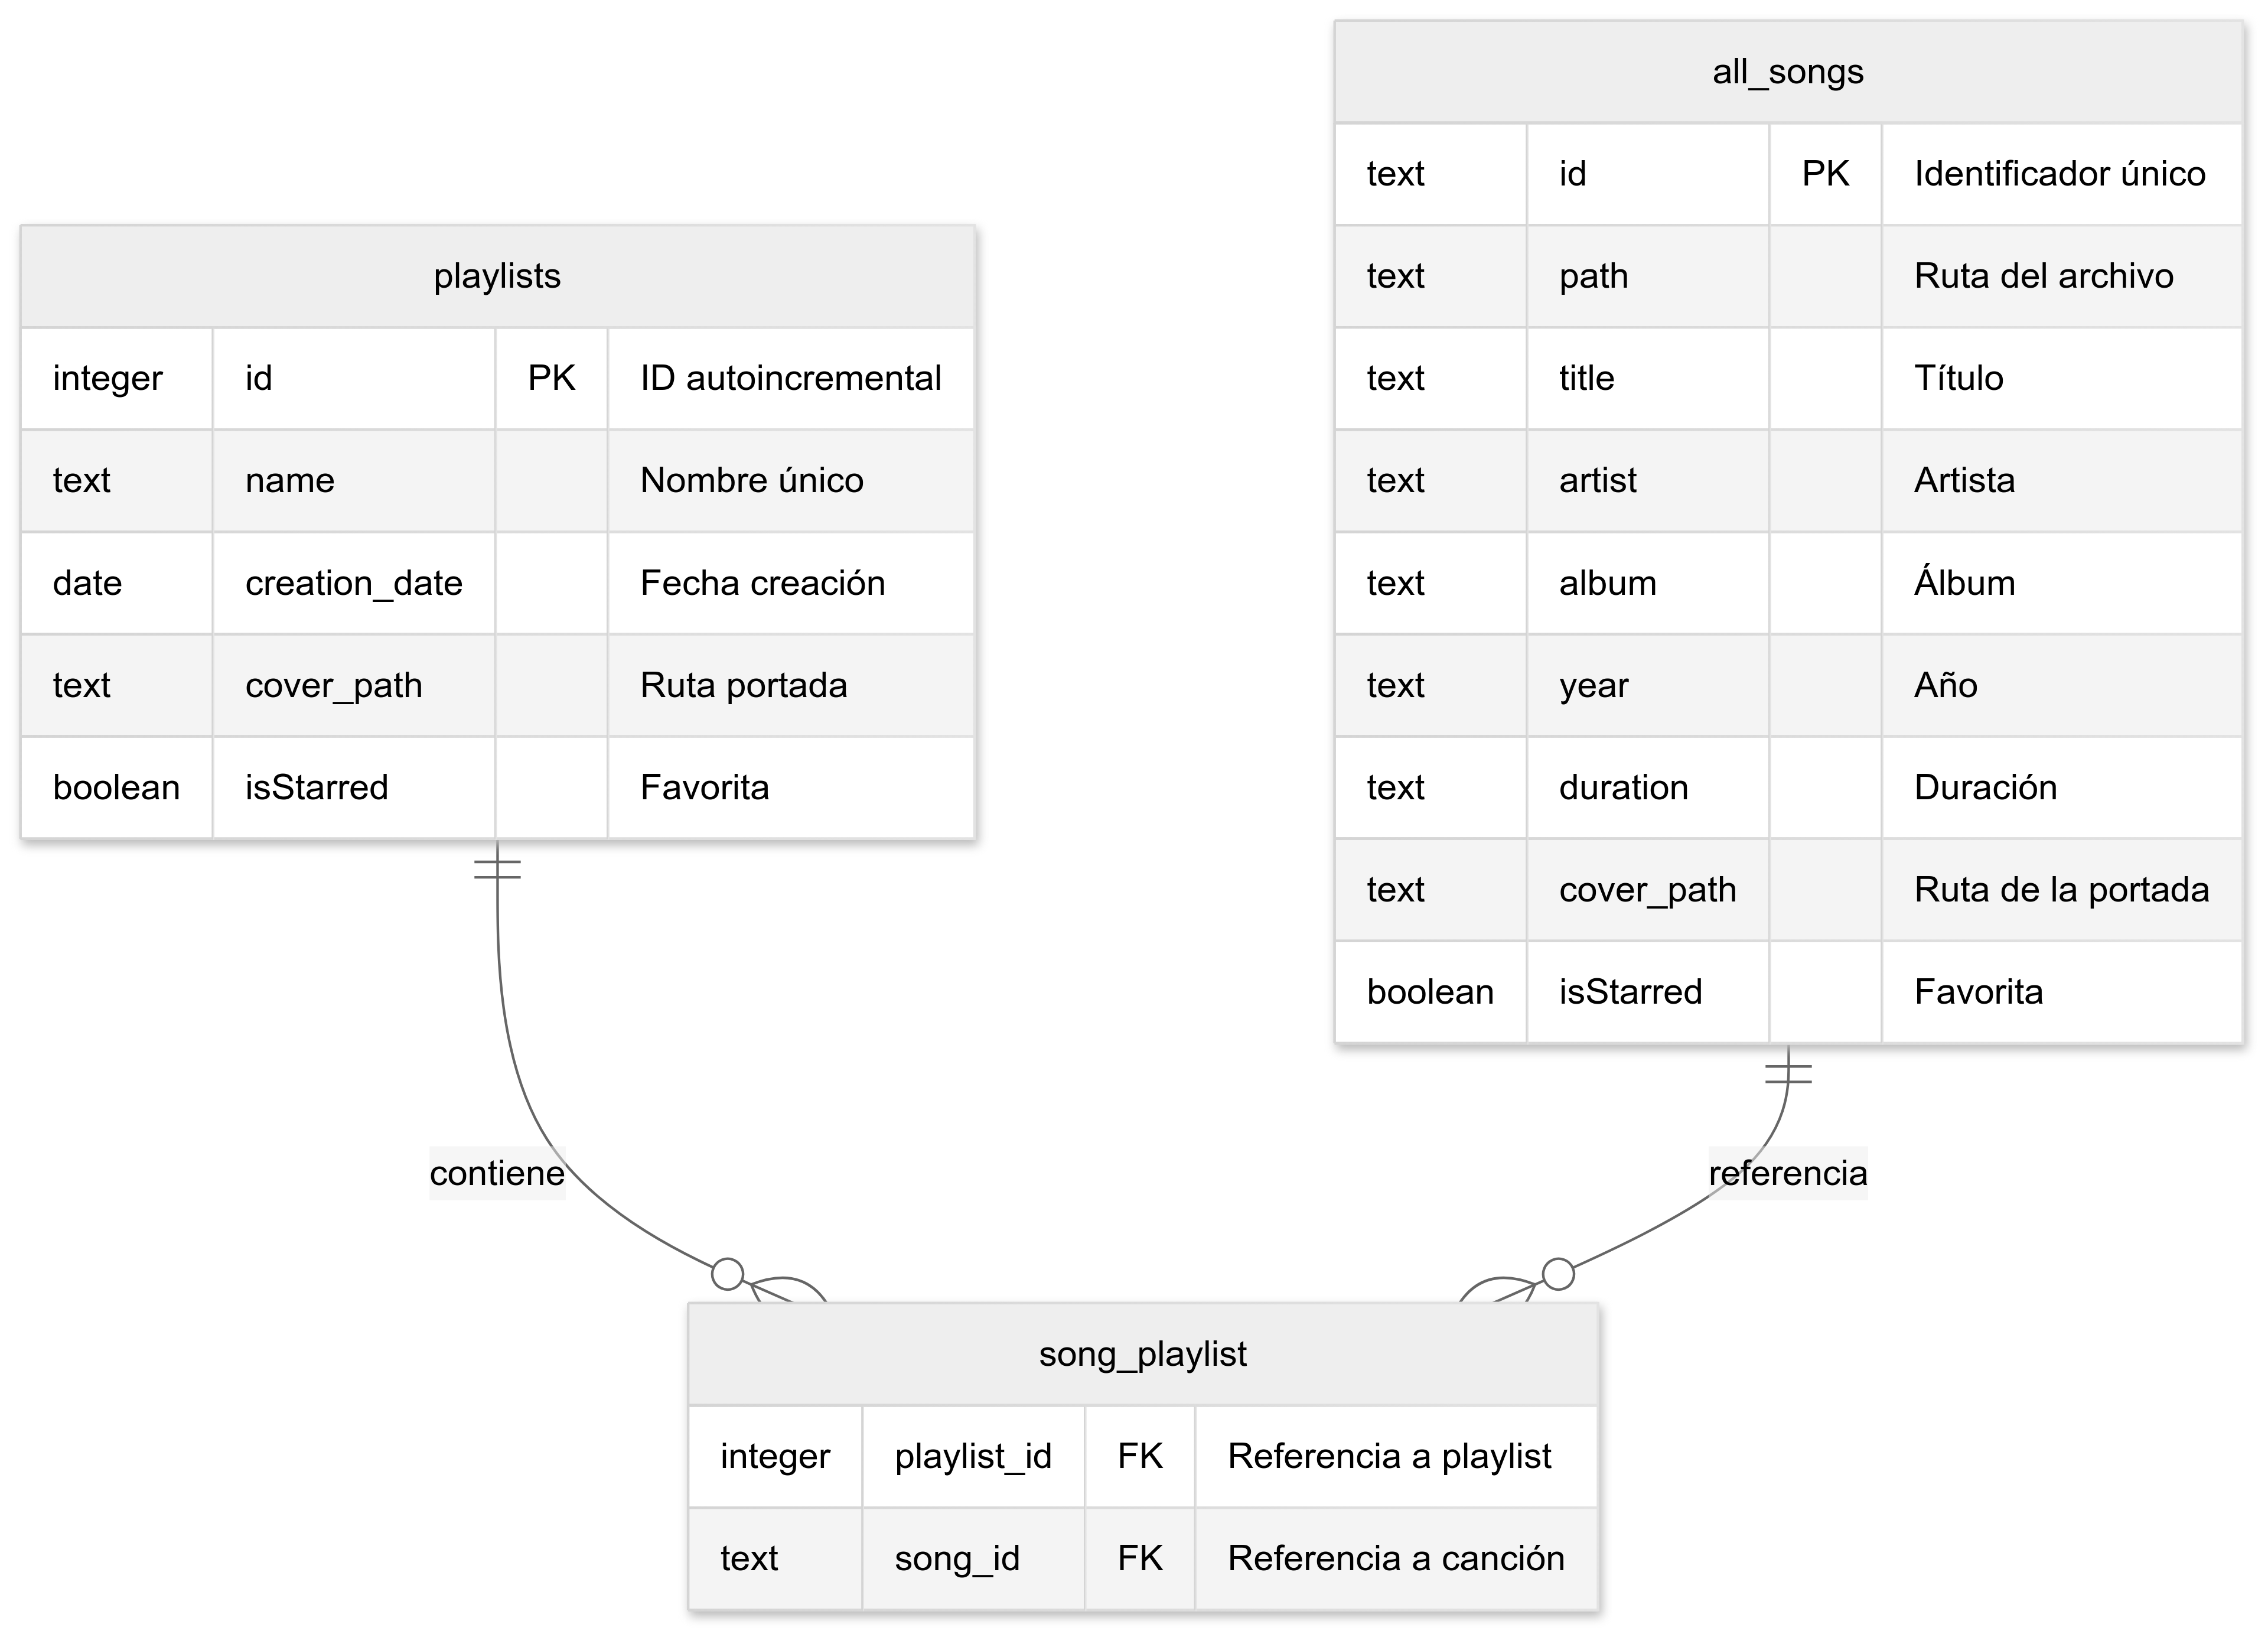
\includegraphics[width=0.8\textwidth]{media/DiagramaRelacional.png}
              \caption{Diagrama Relacional}
              \label{fig:relacional}
            \end{figure}

            La base de datos se ha diseñado como un sistema relacional que gestiona dos entidades principales: las canciones y las listas de reproducción. El esquema sigue los principios de normalización para eliminar redundancias, utilizando una tabla intermedia para manejar la relación \textit{muchos-a-muchos} entre estas entidades.

              \paragraph{All Songs}
              ‎ \\

              Funciona como repositorio central para todas las canciones disponibles en el sistema. Cada registro contiene:

              \begin{itemize}
                \item \textbf{id}: Hash único que actúa como clave primaria.
                \item \textbf{Metadatos}: Incluye título, artista, álbum, y año de lanzamiento.
                \item \textbf{Datos}:  Almacena la ruta del archivo, duración en segundos y ubicación de la portada.
                \item \textbf{isStarred}: Indicador booleano que muestra si la canción ha sido marcada como favorita.
              \end{itemize}

              Esta tabla cumple una función dual como playlist especial (con ID 0 en la tabla de playlists) y presenta características únicas como la imposibilidad de eliminar canciones directamente desde ella.

              \paragraph{Playlist}
              ‎ \\

              Almacena todas las listas de reproducción creadas por los usuarios con los siguientes campos:

              \begin{itemize}
                \item \textbf{id}: Identificador único autoincremental que actúa como clave primaria.
                \item \textbf{Metadatos}: Nombre de la playlist, fecha de creación (formato ISO 8601) y ruta a la imagen de portada (previamente procesada y optimizada).
                \item \textbf{isStarred}: Campo reservado para futuras implementaciones, actualmente no utilizado en la versión 1.0 debido a complejidades en la interacción con la interfaz gráfica.
              \end{itemize}

              \paragraph{Song Playlist}
              ‎ \\

              Establece las relaciones entre canciones y playlists mediante un diseño minimalista que contiene únicamente:

              \begin{itemize}
                \item Clave foránea a \verb|All_Songs.id|.
                \item Clave foránea a \verb|Playlist.id|.
              \end{itemize}

              Esta estructura permite consultas eficientes tanto para recuperar todas las canciones de una playlist como para identificar en qué playlists aparece una canción específica. La integridad referencial se mantiene mediante restricciones \verb|FOREIGN KEY| que garantizan la consistencia de los datos.

            \subsubsection{Logica}

            El módulo \verb|logic.rs| constituye el núcleo funcional del backend, donde se implementan las operaciones críticas de gestión de datos y sincronización musical. Su diseño sigue los principios de Rust: seguridad de tipos, manejo explícito de errores y eficiencia en el acceso a recursos del sistema.

            \begin{lstlisting}[caption={fn sync()}]
pub fn sync(path:PathBuf, music_path:PathBuf) -> std::io::Result<()> {
    create_dir(path.clone())?;
    create_db(path.clone())?;
    clean(path.clone()).unwrap();
    walk_dir(music_path, path.clone())?;

    Ok(())
}
            \end{lstlisting}

            La función \verb|sync()| coordina el proceso completo de inicialización de la biblioteca musical mediante cuatro etapas secuenciales:

            \begin{enumerate}
                \item \textbf{Preparación del entorno}.
                \item \textbf{Inicialización de la base de datos}.
                \item \textbf{Limpieza de registros obsoletos}.
                \item \textbf{Exploración del directorio musical}: \verb|walk_dir| recorre recursivamente la ruta especificada para indexar nuevos archivos.
            \end{enumerate}

            Cada etapa maneja sus errores de forma independiente, siguiendo el patrón \verb|Result| de Rust. La función principal propaga los errores mediante el operador \verb|?|, mientras que \verb|clean| utiliza \verb|unwrap| al considerarse una operación no crítica.

            \begin{lstlisting}[caption={fn create\_dir()}]
fn create_dir(path:PathBuf) -> std::io::Result<()> {
    let new_path = path.join("covers");
    fs::create_dir_all(&new_path).expect("Error");
    Ok(())
}
            \end{lstlisting}

            Esta función se encarga de inicializar la estructura de directorios necesaria para el almacenamiento de archivos auxiliares.

            El proceso sigue tres pasos fundamentales:

            \begin{enumerate}
              \item Construye la ruta completa concatenando el directorio base con la subcarpeta \verb|covers|.
              \item Ejecuta la creación recursiva de directorios mediante \verb|fs::create_dir_all()|.
              \item Maneja posibles errores con \verb|expect| para fallos críticos.
            \end{enumerate}

            La implementación garantiza que exista siempre el directorio para almacenar las portadas de las canciones, requisito esencial para el funcionamiento de la interfaz gráfica. El uso de \verb|PathBuf| en lugar de manipulaciones de strings crudas facilita su uso.

            \begin{lstlisting}[caption={fn create\_db()}]
fn create_db(path:PathBuf) -> std::io::Result<()> {
    let conn = Connection::open(path.join("playlists.db")).expect("Error");
    conn.execute("create table if not exists all_songs(
        id text primary key not null,
        path text not null,
        title text not null,
        artist text,
        album text,
        year text,
        duration text,
        cover_path text,
        isStarred boolean default false
    );",()).expect("ERROR2");

    conn.execute("create table if not exists playlists (
        id integer primary key autoincrement,
        name text not null unique,
        creation_date DATE default CURRENT_DATE,
        cover_path text default '',
        isStarred boolean default false
    )", ()).expect("ERROR3");

    conn.execute("create table if not exists song_playlist(
        playlist_id integer not null,
        song_id text not null,
        foreign key (playlist_id) references playlists(id) ON DELETE CASCADE,
        foreign key (song_id) references all_songs(id) ON DELETE CASCADE,
        primary key (playlist_id, song_id)
    );",() ).expect("ERROR4");

    conn.execute("INSERT OR REPLACE INTO playlists (id, name) VALUES (?1,?2);", (0,"All Songs",)).expect("ERROR WHILE INSERTING");

    Ok(())
}
            \end{lstlisting}

            La función \verb|create_db| genera la estructura SQLite con las tablas necesarias vistas en el punto anterior.

            El diseño utiliza \verb|if not exists| para evitar errores en ejecuciones repetidas y maneja errores mediante el operador \verb|?| de Rust.

            \begin{lstlisting}[caption={fn clean()}]
fn clean(database_path: PathBuf) -> Result<()> {
    let mut conn = Connection::open(database_path.join("playlists.db"))?;

    let rows: Vec<(String, String)> = {
        let mut stmt = conn.prepare("SELECT id, path FROM all_songs")?;
        let rows_iter = stmt.query_map([], |row| {
            Ok((row.get::<_, String>(0)?, row.get::<_, String>(1)?))
        })?;

        let mut collected = Vec::new();
        for row in rows_iter {
            collected.push(row?);
        }
        collected
    };

    let tx = conn.transaction()?;

    for (id, path_str) in rows {
        println!("Checking path: {}", path_str);
        println!("Path exists? {}", Path::new(&path_str).exists()); 
        if !Path::new(&path_str).exists() {
            println!("Removing song: {} - File not found: {}", id, path_str);
            tx.execute("DELETE FROM all_songs WHERE id = ?", [id])?;
        }
    }

    tx.commit()?;
    println!("Operation completed.");
    Ok(())
}
            \end{lstlisting}

            Esta función implementa el mantenimiento de la base de datos eliminando registros de canciones cuyos archivos ya no existen en el sistema.

            La función sigue un flujo de cuatro etapas:

            \begin{enumerate}
              \item \textbf{Consulta inicial}: Recupera todos los IDs y rutas de canciones almacenadas mediante una consulta SQL parametrizada. El uso de \verb|query\_map()| permite un mapeo seguro de los resultados a tuplas Rust.

              \item \textbf{Transacción}: Inicia una transacción SQLite para garantizar atomicidad en las operaciones de limpieza. Esto previene estados inconsistentes si ocurren errores durante el proceso.

              \item \textbf{Verificación}: Para cada canción registrada:
                \begin{itemize}
                  \item Comprueba la existencia del archivo físico usando \verb|Path::exists()|.
                  \item Elimina el registro de la base de datos si el archivo no existe.
                  \item Registra la operación en la consola para diagnóstico.
                \end{itemize}

              \item \textbf{Confirmación}: Finaliza la transacción aplicando todos los cambios de forma atómica.
            \end{enumerate}

            Características técnicas destacables:
            \begin{itemize}
              \item Manejo de errores unificado con el tipo \verb|Result| de Rust.
              \item Uso de transacciones para garantizar integridad de datos.
              \item Consultas parametrizadas para prevenir inyección SQL.
            \end{itemize}

            \begin{lstlisting}[caption={fn walk\_dir()}]
 fn walk_dir(path:PathBuf, data_path:PathBuf) -> std::io::Result<()> {
    for entry in WalkDir::new(&path).into_iter().filter_entry(|e| is_music(e)) {
        let entry = entry?;
        if entry.file_name().to_str().unwrap_or("").ends_with(".mp3") || entry.file_name().to_str().unwrap_or("").ends_with(".ogg") {
            println!("{}", entry.path().display());
            let data = extract_metadata(entry.path().to_str().unwrap(),data_path.join("covers"))?;
            insert_song(data_path.clone(), entry.path().to_string_lossy().to_string(), data.0, data.1, data.2, data.3, data.4, data.5);
        }
    }
    Ok(())
}
            \end{lstlisting}

            Función principal que coordina el recorrido del directorio \textit{music}.

            Utiliza \verb|WalkDir| para recorrido recursivo eficiente y filtra archivos mediante \verb|is_music()| durante el recorrido. Cada archivo válido es procesado con \verb|extract_metadata| y almacenado mediante \verb|insert_song()|.

            \begin{lstlisting}[caption={fn is\_music()}]
fn is_music(entry: &DirEntry) -> bool {
    entry.file_name().to_str().map(|s| {s.ends_with(".mp3") || s.ends_with(".ogg") || s.ends_with(".wav") || s.ends_with(".flac") || s.ends_with(".aac")}).unwrap_or(false) || entry.file_type().is_dir()
}
            \end{lstlisting}

            Filtro para identificar archivos musicales.

            Soporta múltiples formatos de audio incluyendo \verb|.mp3|, \verb|.ogg|, \verb|.wav|, \verb|.flac| y \verb|.aac|. Permite recursividad al incluir directorios mediante \verb|is_dir| con manejo seguro de conversión de nombres de archivo.

            \begin{lstlisting}[caption={fn extract\_metadata()}]
fn extract_metadata(path:&str, cover_path:PathBuf) -> std::io::Result<(String, String, String, String, u128, String)> {
    let tagged_file = read_from_path(path).expect("Error");
    let first_tag = tagged_file.first_tag();
    let title = first_tag.unwrap().title().unwrap().to_string();
    let artist = first_tag.unwrap().artist().unwrap_or(Cow::from("Unkown")).to_string();
    let album = first_tag.unwrap().album().unwrap_or(Cow::from("Unkown")).to_string();
    let year = first_tag.unwrap().year().unwrap_or(0000).to_string();
    let duration = tagged_file.properties().duration().as_millis();
    let cover = first_tag.unwrap().pictures().first().map(|p| p.data().to_vec() );

    let cover_path = create_cover(cover_path, &title, cover).expect("Error creating cover");

    Ok((title,artist,album,year,duration,cover_path.to_string_lossy().to_string()))
}
            \end{lstlisting}

            Extracción de metadatos de archivos musicales.

            Lee metadatos usando la crate \verb|lofty| con valores por defecto para campos opcionales. Convierte la duración a milisegundos y gestiona la extracción de imágenes de portada mediante \verb|create_cover()|.

            \begin{lstlisting}[caption={fn create\_cover()}]
fn create_cover(path:PathBuf, title:&str, image:Option<Vec<u8>>) -> std::io::Result<PathBuf> {

    let hash = blake3::hash(title.as_ref());
    let file_name = format!("{}.jpg",hash);
    let full_path = path.join(file_name);

    let image_data = image.unwrap_or_else(|| DEFAULT_BLACK_IMAGE.to_vec());

    let cover = File::create(&full_path);
    cover?.write_all(image_data.as_ref()).expect("ERROR writing");
    Ok(full_path)
}
            \end{lstlisting}

            Con el propósito de no estar constantemente extrayendo la portada de la canción, se crea un archivo dentro del directorio del programa con un hash como nombre.

            \begin{lstlisting}[caption={fn insert\_song()}]
fn insert_song(path:PathBuf , song_path:String, title:String, artist:String, album:String, year:String, duration: u128, cover_path:String) {
    let dur_secs = (duration / 1000) as i64;
    let new_duration = format!("{}:{:02}",dur_secs / 60, dur_secs % 60);
    let uuid = blake3::hash(title.as_ref());

    let conn = Connection::open(path.join("playlists.db")).expect("Error");
    conn.execute("INSERT OR IGNORE INTO all_songs (id, path, title, artist, album, year, duration, cover_path) VALUES (?1,?2,?3,?4,?5,?6,?7,?8);", (uuid.to_string(), song_path, title, artist, album, year, new_duration, cover_path)).expect("ERROR WHILE INSERTING");
}
            \end{lstlisting}

            Genera ID único mediante hash Blake3 del título usando \verb|blake3::hash()|. Formatea la duración a \verb|MM:SS| y evita duplicados con \verb|INSERT OR IGNORE|. Almacena todos los metadatos extraídos en la tabla \verb|all_songs| de la base de datos SQLite.

            \begin{lstlisting}[caption={Operaciones CRUD playlist}]
pub fn add_playlist(name:String, cover_path:String, db_path:String) -> Result<()> {
    let conn = Connection::open(PathBuf::from(db_path).join("playlists.db"))?;

    conn.execute("INSERT INTO playlists (name, cover_path) VALUES (?1, ?2);", (name, cover_path)).expect("ERROR WHILE INSERTING");

    Ok(())
}

pub fn remove_a_playlist(playlist_id:i64, db_path:String) -> Result<()> {
    let conn = Connection::open(PathBuf::from(db_path).join("playlists.db"))?;

    conn.execute("DELETE FROM playlists WHERE id = ?1",(playlist_id,)).expect("ERROR WHILE DELETING SONG");

    Ok(())
}
            \end{lstlisting}

            Métodos encargados de crear y eliminar \textit{playlists} de la base de datos. Primero se crea una conexión y posteriormente se ejecuta la consulta con los parámetros de la playlist.

            \begin{lstlisting}[caption={Operaciones CRUD canciones}]
pub fn add_song(playlist_id:i64, song_id:String, db_path:String) -> Result<()> {
    let conn = Connection::open(PathBuf::from(db_path).join("playlists.db"))?;

    conn.execute("INSERT OR REPLACE INTO song_playlist (playlist_id, song_id) VALUES (?1,?2);",(playlist_id, song_id)).expect("ERROR WHILE INSERTING SONG");

    Ok(())
}

pub fn remove_song(playlist_id:i64, song_id:String, db_path:String) -> Result<()> {
    let conn = Connection::open(PathBuf::from(db_path).join("playlists.db"))?;

    conn.execute("DELETE FROM song_playlist WHERE playlist_id = ?1 AND song_id = ?2",(playlist_id, song_id)).expect("ERROR WHILE DELETING SONG");

    Ok(())
}

pub fn add_starred(song_id:String, db_path:String) -> Result<()> {
    let conn = Connection::open(PathBuf::from(db_path).join("playlists.db"))?;

    conn.execute("UPDATE all_songs SET isStarred = 1 WHERE id = ?",(song_id,)).expect("ERROR WHILE MODIFIYING STARRED");

    Ok(())
}

pub fn remove_starred(song_id:String, db_path:String) -> Result<()> {
    let conn = Connection::open(PathBuf::from(db_path).join("playlists.db"))?;

    conn.execute("UPDATE all_songs SET isStarred = 0 WHERE id = ?",(song_id,)).expect("ERROR WHILE MODIFIYING STARRED");

    Ok(())
}
            \end{lstlisting}

            Métodos encargados de crear, eliminar y actualizar canciones de la base de datos. Primero se crea una conexión y posteriormente se ejecuta la consulta con los parámetros de la canción. Para las canciones favoritas se ejecuta es una consulta de \verb|UPDATE|.

            La implementación de los siguientes métodos utilizan estos \verb|struct|s:

            \begin{lstlisting}[caption={structs Song y Playlist}]
pub struct Song {
  id: String,
  path: String,
  title: String,
  artist: String,
  album: String,
  year: String,
  duration: String,
  #[serde(rename = "coverPath")]
  cover_path: String,
  #[serde(rename = "isStarred")]
  is_starred: bool,
}

pub struct Playlist {
  id: i64,
  name: String,
  creation_date: String,
  cover_path: String,
  #[serde(rename = "isStarred")]
  is_starred: bool,
}
            \end{lstlisting}

            El \verb|struct| \verb|Song| contiene todos los datos relevantes de cada canción ya vistos en la sección de la base de datos, incluyendo:

            \begin{itemize}
              \item Identificador único (\verb|id|).
              \item Ruta del archivo (\verb|path|).
              \item Metadatos (\verb|title|, \verb|artist|, \verb|album|, \verb|year|).
              \item Información de reproducción (\verb|duration|).
              \item Ruta de la portada (\verb|cover_path|).
              \item Estado (\verb|is_starred|).
            \end{itemize}

            Por otra parte, \verb|Playlist| incluye:

            \begin{itemize}
              \item Identificador único (\verb|id|).
              \item Nombre de la \textit{Playlist} (\verb|name|).
              \item Fecha de creación (\verb|creation_date|).
              \item Portada (\verb|cover_path|).
              \item Estado (\verb|is_starred|, no implementado por el momento).
            \end{itemize}

            \begin{lstlisting}[caption={fn get\_all\_playlists()}]
pub fn get_all_playlists(db_path:String) -> Result<Vec<Playlist>, String> {
    let conn = Connection::open(PathBuf::from(db_path).join("playlists.db")).map_err(|e| e.to_string())?;

    let mut stmt = conn.prepare("SELECT id, name, creation_date, cover_path, isStarred FROM playlists").map_err(|e| e.to_string())?;

    let playlists = stmt.query_map([], |row| {
        Ok(Playlist {
            id: row.get(0)?,
            name: row.get(1)?,
            creation_date: row.get(2)?,
            cover_path: row.get(3)?,
            is_starred: row.get(4)?,
        })
    }).map_err(|e| e.to_string())?
    .collect::<Result<Vec<_>, _>>()
    .map_err(|e| e.to_string())?;

    Ok(playlists)
}
            \end{lstlisting}

            Esta función implementa la consulta de todas las playlists almacenadas en la base de datos.

            El proceso se ejecuta en tres etapas principales. Primero se establece la conexión con la base de datos ubicada en \verb|playlists.db| dentro del directorio especificado.

            Seguidamente se prepara y ejecuta la consulta SQL que selecciona todos los campos de la tabla \verb|playlists|.

            Finalmente, los resultados son mapeados a instancias del \verb|struct| \verb|Playlist| mediante un \verb|query_map()| que procesa cada fila. El mapeo incluye todos los campos relevantes: \verb|id|, \verb|name|, \verb|creation_date|, \verb|cover_path| y \verb|is_starred|.

            El vector resultante con todas las playlists es devuelto al frontend a través de \verb|lib.rs|, donde será utilizado para poblar la interfaz de usuario como se ha visto previamente en esta documentación.

            \begin{lstlisting}[caption={fn get\_all\_songs() y fn get\_all\_songs\_starred()}]
pub fn get_all_songs(db_path:String) -> Result<Vec<Song>, String> {
    let conn = Connection::open(PathBuf::from(db_path).join("playlists.db")).map_err(|e| e.to_string())?;

    let mut stmt = conn.prepare("SELECT id, path, title, artist, album, year, duration, cover_path, isStarred FROM all_songs").map_err(|e| e.to_string())?;

    let all_songs = stmt.query_map([], |row| {
        Ok(Song {
            id: row.get(0)?,
            path: row.get(1)?,
            title: row.get(2)?,
            artist: row.get(3)?,
            album: row.get(4)?,
            year: row.get(5)?,
            duration: row.get(6)?,
            cover_path: row.get(7)?,
            is_starred: row.get(8)?,
        })
    }).map_err(|e| e.to_string())?
    .collect::<Result<Vec<_>, _>>()
    .map_err(|e| e.to_string())?;

    Ok(all_songs)

}

pub fn get_all_songs_starred(db_path:String) -> Result<Vec<Song>, String> {
    let conn = Connection::open(PathBuf::from(db_path).join("playlists.db")).map_err(|e| e.to_string())?;

    let mut stmt = conn.prepare("SELECT id, path, title, artist, album, year, duration, cover_path, isStarred FROM all_songs WHERE isStarred = 1").map_err(|e| e.to_string())?;

    let all_songs = stmt.query_map([], |row| {
        Ok(Song {
            id: row.get(0)?,
            path: row.get(1)?,
            title: row.get(2)?,
            artist: row.get(3)?,
            album: row.get(4)?,
            year: row.get(5)?,
            duration: row.get(6)?,
            cover_path: row.get(7)?,
            is_starred: row.get(8)?,
        })
    }).map_err(|e| e.to_string())?
    .collect::<Result<Vec<_>, _>>()
    .map_err(|e| e.to_string())?;

    Ok(all_songs)
}
            \end{lstlisting}

            Estas funciones implementan el acceso a las canciones almacenadas en la base de datos, ambas comparten la misma estructura pero tienen un propósito diferente.

            \verb|get_all_songs()| recupera todas las canciones almacenadas en la tabla \verb|all_songs|, mientras que \verb|get_all_songs_starred()| filtra solo aquellas marcadas como favoritas mediante la condición \verb|WHERE isStarred = 1|.

            El flujo de ejecución es idéntico en ambos casos:
            \begin{enumerate}
              \item Establece conexión con la base de datos.
              \item Prepara y ejecuta la consulta SQL correspondiente.
              \item Mapea los resultados a instancias del \verb|struct| \verb|Song|.
              \item Devuelve el vector de canciones o propaga cualquier error.
            \end{enumerate}

            \begin{lstlisting}[caption={fn get\_playlist\_songs()}]
pub fn get_playlist_songs(playlist_id: i64, db_path: String) -> Result<Vec<Song>, String> {
    let conn = Connection::open(PathBuf::from(db_path).join("playlists.db"))
        .map_err(|e| e.to_string())?;

    let mut stmt = conn.prepare(
        "SELECT s.id, s.path, s.title, s.artist, s.album, s.year, s.duration, s.cover_path, s.isStarred FROM all_songs s INNER JOIN song_playlist sp ON s.id = sp.song_id WHERE sp.playlist_id = ?1"
    ).map_err(|e| e.to_string())?;

    let playlist_songs = stmt
        .query_map([playlist_id], |row| {
            Ok(Song {
                id:          row.get(0)?,
                path:        row.get(1)?,
                title:       row.get(2)?,
                artist:      row.get(3)?,
                album:       row.get(4)?,
                year:        row.get(5)?,
                duration:    row.get(6)?,
                cover_path:  row.get(7)?,
                is_starred:  row.get(8)?,
            })
        })
        .map_err(|e| e.to_string())?
        .collect::<Result<Vec<_>, _>>()
        .map_err(|e| e.to_string())?;

    Ok(playlist_songs)
}
            \end{lstlisting}

            Esta función implementa la consulta de canciones pertenecientes a una playlist específica mediante una operación JOIN.

            La función realiza una consulta SQL compleja que combina los datos de las tres tablas:

            \begin{itemize}
              \item \verb|all_songs|: Contiene los metadatos completos de las canciones.
              \item \verb|song_playlist|: Establece las relaciones entre canciones y playlists.
            \end{itemize}

            El JOIN se realiza mediante la condición \verb|s.id = sp.song_id|, filtrando por el parámetro \verb|playlist_id| proporcionado.

            Los campos seleccionados incluyen todos los metadatos necesarios para la reproducción y visualización al igual que en los métodos anteriores:
            \begin{itemize}
              \item Identificación única (\verb|id|)
              \item Ruta del archivo (\verb|path|)
              \item Metadatos (\verb|title|, \verb|artist|, \verb|album|, \verb|year|)
              \item Duración formateada (\verb|duration|)
              \item Ruta de la portada (\verb|cover_path|)
              \item Estado (\verb|isStarred|)
            \end{itemize}

\section{Conclusiones}

        \subsection{Logros principales}

        Se ha desarrollado con éxito un reproductor de música multiplataforma (Linux, MacOs y Windows) utilizando Tauri, que cumple con los objetivos principales de:

        \begin{itemize}
            \item Optimización de recursos (Mucho menor consumo de ram respecto a otras webapps basadas en Electro).
            \item Compatibilidad de formatos de audio (FLAC, MP3, etc...).
            \item Arquitectura modular para el desarrollo futuro.
        \end{itemize}

        \subsection{Dificultades clave}

        El principal desafío técnico fue la curva de aprendizaje asociada a Rust, lenguaje de programación de sistemas con el que no se contaba experiencia previa. Esta dificultad se resolvió mediante el estudio de documentación oficial, tutoriales especializados y la implementación de pruebas piloto. Adicionalmente, fue necesario adaptar los conocimientos existentes en desarrollo web al framework Angular, cuyo paradigma de componentes requirió un período de adaptación.

        \subsection{Valoración global}

        A pesar de las dificultades, el proyecto valida el potencial de Tauri para aplicaciones de audio eficientes, ofreciendo un rendimiento superior al de frameworks tradicionales. La escalabilidad de la arquitectura permite añadir funcionalidades como cambios en la apariencia en futuras iteraciones.

          \subsubsection{Paginas webs visitadas durante el desarrollo}

          \begin{itemize}
            \item \textcite{angular2025} Documentación de Angular.
            \item \textcite{cursoangular2025} Curso web de Angular.
            \item \textcite{fontawesome} Iconos.
            \item \textcite{lofty} Audio en Rust.
            \item \textcite{mdnarraybuffer}
            \item \textcite{mdnblob}
            \item \textcite{mdncanvas}
            \item \textcite{mdnpadStart}
            \item \textcite{rusqlite} Bases de datos en Rust.
            \item \textcite{stackoverflowshuffle}
            \item \textcite{tailwind2025} Estilo de HTML.
            \item \textcite{tauri2024} Base del programa.
            \item \textcite{walkdir} Recorrer directorios en Rust.
            \item \textcite{youtuberust2024} Aprendizaje de Rust
            \item \textcite{mermaid} Para la creación de Diagramas.
          \end{itemize}
\printbibliography
\end{document}